\documentclass[11pt]{article}
\usepackage[margin=1in]{geometry}
\usepackage{amsmath,amssymb,amsthm}
\usepackage{booktabs}
\usepackage{enumitem}
\usepackage{flafter}
\usepackage{graphicx}
\usepackage{placeins}
\usepackage[hidelinks]{hyperref}
\setlist[itemize]{leftmargin=1.4em}
\setlist[enumerate]{leftmargin=1.6em}
\newcommand{\KL}{D}
\newcommand{\E}{\mathbb{E}}
\newcommand{\Nseq}{N}
\newcommand{\model}{\mathcal{M}_{d,L}}
\newtheorem{proposition}{Proposition}
\newtheorem{remark}{Remark}
\usepackage{xcolor}
\newcommand{\cstar}{c^{\star}}
% --- notation macros: one place to change any contested symbol ---
\newcommand{\batchreg}{R^{\mathrm{B}}} % batch regret (frees B for B(c,alpha))
\newcommand{\price}{\rho}            % price per bit of description (was A(c))
\newcommand{\rate}{I}                % Legendre transform of log Gamma(1+s) (was Lambda^*)
\newcommand{\op}{\omega}             % order parameter (was phi(theta))
\newcommand{\Mlab}{M_{\mathrm{lab}}} % relabeling count (was M(theta_0))
\usepackage{tikz}
\usetikzlibrary{decorations.pathreplacing,arrows.meta}
\title{A Layered Simplex Architecture for Large Alphabets}

\author{
  Meir Feder and Yaniv Fogel\\
  School of Electrical and Computer Engineering\\
  Tel Aviv University, Tel Aviv, Israel\\
  \texttt{meir@tau.ac.il}, \texttt{yaniv.fogel8@gmail.com}
  \and
  Ruediger Urbanke\\
  School of Computer and Communication Sciences\\
  EPFL, Lausanne, Switzerland\\
  \texttt{rudiger.urbanke@epfl.ch}
}

\date{\today}

\begin{document}
\maketitle
\begin{abstract}
Probability estimation over large alphabets under log loss is a well-studied problem, with celebrated methods such as the Good--Turing estimator. We introduce and study a new Bayesian estimator with four notable properties. First, its construction is exceptionally simple: multiply independent uniform draws from the probability simplex coordinate-wise and renormalize. Depth is the only structural parameter, and averaging over depths eliminates the need to tune it. Second, the regret of the resulting mixture, the excess code length it pays
relative to a code that knows the source, admits an explicit and efficiently
computable expression. Third, despite its simplicity and lack of tuned constants, the estimator is competitive across a diverse set of synthetic and real-text benchmarks with substantially more specialized methods, including Good--Turing.
Fourth, the tractability of its regret allows us to identify scaling
laws in data, alphabet size, and depth. For Zipf targets with exponent
above one, the regret has a simple reading as long as the
sample reveals only a small fraction of the alphabet. It closely matches the
description length of the set of discovered symbols, at one bit of code per
bit of description, plus a further cost per symbol. The data exponent is
therefore the rate at which new symbols are discovered.
\end{abstract}

\section{Introduction}
\label{sec:intro}
Three questions motivate this paper.

\emph{First}, can a simple Bayesian estimator compete in the
large-alphabet regime?
Estimating an unknown distribution under log loss is a classical problem,
but it becomes particularly difficult when the alphabet size $d$ is large relative to the available data $N$.
Simple Bayesian rules with uniform prior over the $d$ dimensional simplex leads to the add-one rule (Laplace) and with Dirichlet $1/2$ prior to the the add-half rule
(Krichevsky--Trofimov~\cite{krichevsky1981performance}); both spread probability
across the entire alphabet and can therefore perform poorly when the target
is sparse or heavy-tailed.
Good--Turing estimation~\cite{good1953population} and its variants address
this regime well, with strong guarantees in several competitive
frameworks~\cite{orlitsky2003always,mcallester2000leave,acharya2013tight,
orlitsky2015competitive}.
Ristad's natural law of succession~\cite{ristad1995natural} indicates that a
hierarchical construction can recover some of this adaptivity.
We ask whether a simple Bayesian construction can compete with these more
specialized estimators across both flat and highly concentrated targets.
Its only structural parameter is the depth, and even that can be removed
by averaging over it.

\emph{Second}, can the scaling of such an estimator be understood from
first principles?
Empirical scaling laws in machine learning describe robust power-law
improvements with data, model size, and compute~\cite{kaplan2020scaling},
but their exponents are generally difficult to derive.
Large-alphabet estimation offers a setting in which the relevant mechanism
may be isolated: under a heavy-tailed source, the number of distinct symbols
revealed by the data itself follows a scaling law.
A nontrivial but tractable estimator could therefore connect its regret
directly to the rate of symbol discovery, providing a solvable example in
which the origin of a scaling exponent is explicit.

\emph{Third}, what does a layered architecture buy?
In the information-theoretic view of machine learning developed
in~\cite{feder2025framework}, an architecture together with the randomness
of its initialization induces a prior \(w\) over predictors.
The corresponding Bayesian mixture pays, on a particular target, according
to how much prior mass lies near that target: up to lower-order terms, its
regret is governed by
\[
    -\log w\bigl(\Theta_0^\epsilon\bigr),
\]
the negative logarithm of the prior mass of a small neighborhood of the
best predictor~\cite{feder1992universal,MerhavFeder1998,
feder2025framework}.
Layered architectures can induce priors with a broad complexity range:
multiplying independent random factors spreads their sizes over many
orders of magnitude, so appreciable prior mass lands on predictors of
very different complexities.
Can this mechanism be exhibited in a minimal model in which the prior,
regret, and resulting scaling laws can all be computed?

We answer these questions using the prior induced by a layered simplex
architecture (LSA) on the alphabet \(\mathcal X_d=\{1,\ldots,d\}\); we
call it the LSA prior and its Bayesian mixture the LSA predictor.
At depth \(L\), we draw \(L\) independent uniform points $\{U_i\}_{i=1}^L$ from the
probability simplex, multiply them coordinatewise, and renormalize:
\[
  \theta_i
  =
  \frac{\prod_{\ell=1}^L U^{(\ell)}_i}
       {\sum_{j=1}^d \prod_{\ell=1}^L U^{(\ell)}_j},
  \qquad i=1,\ldots,d.
\]
Sometimes, such multiplication and normalization is called ``product of experts'' \cite{Hinton1999ProductsOE}. This leads to a non-uniform LSA prior on the $d$-dimensional simplex. With this prior, we can perform a Bayesian mixture over $P_\theta(x^N)$ a multinomial distribution, to get $Q_N^{(L)}(x^N)$, which will define the LSA predicitor. The construction has only one structural parameter.
At \(L=1\), its Bayesian mixture is exactly Laplace's add-one rule; at depth
proportional to \(\ln d\), typical prior draws become sparse and
heavy-tailed.
Because different depths favor targets of different concentration, we also
study a predictor that averages the mixtures over all depths up to a maximum
\(L_{\max}\):
\begin{equation}
\label{eq:depth-average}
  Q^{\mathrm{avg}}_\Nseq(x^\Nseq)
  \;=\;
  \frac{1}{L_{\max}}\sum_{L=1}^{L_{\max}} Q^{(L)}_\Nseq(x^\Nseq).
\end{equation}
The result is a single coherent Bayesian predictor that requires no depth
selection and automatically shifts its posterior weight toward the depths
best suited to the observed data.
Thus the same model provides a competitive large-alphabet estimator, a
tractable setting for studying scaling laws, and a minimal example of a
layered prior with a broad complexity range.

\paragraph{Contributions.}
\begin{enumerate}
\item \emph{An exact and computable regret.}  We derive an exact expression
  for the regret as a sum over the possible \emph{profiles} of the sample,
  where the profile records how many symbols were observed once, how many
  twice, and so on (but not which symbols):
  \[
    R_\Nseq
    =
    -H(p)
    -
    \frac1\Nseq\sum_{\lambda\in\Lambda_\Nseq}
    A_\lambda(p)\log_2 q_\lambda .
  \]
  The formula separates the two ingredients of the problem:
  \(A_\lambda(p)\) depends only on the target, \(q_\lambda\) only on the
  architecture.  At depth \(L=1\) the induced predictor is exactly
  Laplace's add-one rule (Proposition~\ref{prop:laplace}), so the shallow
  end of the family is a classical baseline.  The expression is efficiently
  computable at scale: we evaluate it for alphabets up to \(d=10^6\),
  depths up to \(L=138\), and up to the \(9\cdot10^5\)-token corpus of
  Section~\ref{sec:bible}.
\item \emph{Deeper priors suit more concentrated targets, and averaging
  over depth removes the need to choose.}  Evaluating every integer depth
  up to \(c=L/\ln d\approx10\) at \(d=10^3,10^4,10^6\), we find that the
  best depth grows with the concentration of the target and with the
  alphabet size; on the most concentrated target at \(d=10^6\) the regret
at the best depth is about \(49\) times smaller than at \(L=1\), while
on the uniform target the ordering reverses
(Section~\ref{sec:spectrum}). The
  depth-averaged predictor \eqref{eq:depth-average} tracks the best single
  depth to within \((\log_2 L_{\max})/\Nseq\) bits per symbol on every
  target, so no depth selection is needed.
\item \emph{A scaling law with an identifiable mechanism.}  For Zipf
  targets with \(\alpha>1\) at logarithmic depth, the regret follows
  \(R_\Nseq\approx C(c,\alpha)\,(\log_2 d)\,\Nseq^{-(1-1/\alpha)}\)
  (Section~\ref{sec:scaling}).  The mechanism is symbol discovery: a
  sample of size \(\Nseq\) reveals about \(\Nseq^{1/\alpha}\) distinct
  symbols, and the prior pays the number of bits needed to say which
  symbols these are, at one bit of code per bit of description, plus a
  premium per discovered symbol.  We both measure this unit price and
  derive it: as a function of the depth coefficient \(c\), it has a flat
  minimum of exactly one at the freezing transition \(\cstar\) of the
  prior---the depth beyond which a typical draw concentrates its mass on a
  few symbols---which is also why the transition leaves no kink in the
  regret.  The data exponent \(1-1/\alpha\) is thus the rate at which new
  symbols are discovered.
\item \emph{The depth-averaged predictor competes with the best classical
  estimators.}  On a benchmark of eleven targets of very different shapes
  (support \(d=10^4\), extending \cite{orlitsky2015competitive}), one
  fixed prior with no tuned constants performs about as well as whichever
  classical method is best for each target: it coincides with add-one on
  the flat targets, matches Good--Turing on Zipf \(\alpha=1.5\), beats it
  on the more concentrated targets, and loses clearly only on the flattest
  ones, where Good--Turing exploits count-frequency statistics that no
  exchangeable mixture in this family uses
  (Section~\ref{sec:comparison}).  On a real text, the entire King James
  Bible over a fixed \(d=10^5\) vocabulary, it is the best method tested
  at every prefix length, with a posterior over depths that stays in the
  logarithmic regime (Section~\ref{sec:bible}).  Adding memory as a second
  architectural axis gains a further \(1.47\) bits per token, while the ordering reverses for flat priors: per-state KT codes worse than the memoryless layered
  model, so at this alphabet size the marginal prior matters more than the
  memory it feeds (Section~\ref{sec:memory}).
\item \emph{Certified computation.} All probabilities are evaluated from
explicit formulas rather than by running the predictor sequentially;
the only statistical error is the Monte Carlo average over count
profiles, whose standard errors are reported. The implementation is
validated against closed forms, independent quadrature, and exact
identities (Appendices~\ref{sec:app-mixture-terms}
and~\ref{sec:app-validation}).
\end{enumerate}
Throughout, regret and KL divergences are reported in bits; asymptotic
formulas use \(\ln d\), which changes only constants.
\section{The Information-Theoretic Setting, in Brief}
\label{sec:framework}
This work is an instance of a general program: the information-theoretic
approach to modern machine learning, in which an architecture with randomly
initialized parameters is analyzed as a \emph{prior over predictors} and
learning as universal prediction \cite{feder1992universal,MerhavFeder1998,feder2025framework}.
We state here the two facts from that setting that the rest of the paper
uses, and return to the setting itself, and to what our results say about
it, in Section~\ref{sec:broader}.
Consider batch or online prediction of a sequence \(x^\Nseq\) under log-loss.
A hypothesis class \(\{p_\theta\}_{\theta\in\Theta}\) with a prior \(w\) over
\(\Theta\) defines the Bayesian mixture
\(Q_\Nseq(x^\Nseq)=\int w(d\theta)\,p_\theta(x^\Nseq)\), the universal
predictor of the class.  For any reference \(\theta_0\) and any neighborhood
\(\Theta_0^{\epsilon}=\{\theta:\ \tfrac1\Nseq
\KL(p_{\theta_0}^\Nseq\|p_\theta^\Nseq)\le\epsilon\}\), the mixture's
per-symbol redundancy against \(p_{\theta_0}\) satisfies the non-uniform bound
\begin{equation}
\label{eq:prior-mass-bound}
  \frac1\Nseq\,\KL\!\left(p_{\theta_0}^\Nseq\,\middle\|\,Q_\Nseq\right)
  \;\le\;
\min_{\epsilon > 0}  \left[ \epsilon
  \;-\;
  \frac1\Nseq\log w\!\left(\Theta_0^{\epsilon}\right) \right ],
\end{equation}
so the price of universality for a \emph{particular} target is governed by
the log prior mass near that target, not by the cardinality or dimension of
the class \cite{feder1992universal,MerhavFeder1998,feder2025framework}.  The quantity
\(-\log w(\Theta_0^{\epsilon})\) is the \emph{complexity of the target under
the prior}; for smooth parametric families it recovers the familiar
\(\frac{k}{2}\log \Nseq\) with \(k\) the (effective) dimension, but in general
it is a property of the prior’s geometry.
An architecture converts the randomness of its initialization into a random
predictor, and the distribution of that random predictor is exactly the
prior \(w\); one claim in \cite{feder2025framework} that this paper makes
exact is that \emph{layered} architectures induce priors with a \emph{broad
complexity range}: the unit of prior mass is spread over the whole range of
complexities, with no level absorbing almost all of it, so that each target
is charged roughly its own complexity.  The LSA is
designed to be, plausibly, the simplest nontrivial instance in which all
the objects in \eqref{eq:prior-mass-bound} (mixture, prior mass, and
regret) can be computed essentially exactly.
\section{The LSA and Its Exact Regret}
\label{sec:model}
Let
\[
  \mathcal X_d=\{1,\ldots,d\},
  \qquad
  \Delta_d=\Bigl\{p\in[0,1]^d:\ \textstyle\sum_{i=1}^d p_i=1\Bigr\}.
\]
Zipf targets serve as a one-parameter family of test distributions.  For
\(\alpha\ge 0\),
\[
  p_i=p_{d,\alpha}(i)
  =
  \frac{i^{-\alpha}}{H_{d,\alpha}},
  \qquad
  H_{d,\alpha}=\sum_{j=1}^d j^{-\alpha},
\]
with \(\alpha=0\) the uniform distribution and larger \(\alpha\) more
concentrated targets.
The prior is a probability distribution over \(\Delta_d\), constructed as
follows. Fix an integer \(L\ge 1\). Draw
\[
  U^{(1)},\ldots,U^{(L)}
  \stackrel{\mathrm{iid}}{\sim}
  \operatorname{Dirichlet}(1,\ldots,1),
\]
multiply the \(L\) simplex points coordinatewise, and renormalize:
\[
  \theta_i
  =
  \frac{\prod_{\ell=1}^L U^{(\ell)}_i}
       {\sum_{j=1}^d \prod_{\ell=1}^L U^{(\ell)}_j},
  \qquad i=1,\ldots,d.
\]
The law of \(\theta\) is denoted \(\model\).  Equivalently, if
\(E_{\ell i}\stackrel{\mathrm{iid}}{\sim}\operatorname{Exp}(1)\), then
\begin{equation}
\label{eq:exp-rep}
  Y_i=\prod_{\ell=1}^L E_{\ell i},
  \qquad
  \theta_i=\frac{Y_i}{\sum_{j=1}^d Y_j},
\end{equation}
because a uniform Dirichlet vector is a normalized vector of iid
exponentials and the simplex normalizations cancel in the final
renormalization.  This LSA construction is shown in Figure~\ref{fig:construction}.
\begin{figure}[htp]
  \centering
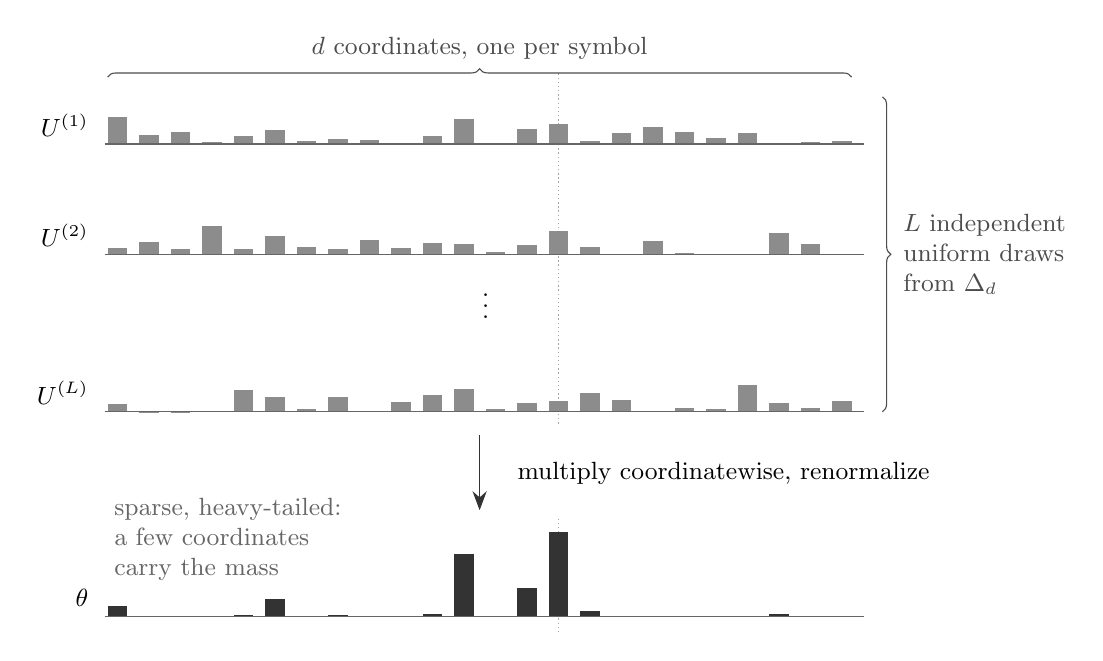
\begin{tikzpicture}[x=4.0mm,y=1mm]
  % dotted guide through the winning coordinate (drawn in two segments)
  \draw[black!35,densely dotted,line width=0.5pt] (15.31,8.5) -- (15.31,53);
  \draw[black!35,densely dotted,line width=0.5pt] (15.31,-18) -- (15.31,-3.5);
  % --- layer rows ---
  \foreach \i/\h in {1/3.43,2/1.21,3/1.53,4/0.21,5/1.02,6/1.72,7/0.35,8/0.65,9/0.53,10/0.19,11/0.99,12/3.15,13/0.07,14/1.94,15/2.54,16/0.40,17/1.39,18/2.11,19/1.47,20/0.78,21/1.44,22/0.14,23/0.30,24/0.43} \fill[black!45] (\i,44) rectangle ++(0.62,\h);
  \draw[black!60,line width=0.4pt] (0.9,44) -- (25.0,44);
  \node[left,font=\small] at (0.7,46.4) {$U^{(1)}$};
  \foreach \i/\h in {1/0.86,2/1.58,3/0.63,4/3.58,5/0.63,6/2.27,7/0.98,8/0.65,9/1.81,10/0.77,11/1.44,12/1.33,13/0.23,14/1.22,15/2.95,16/0.94,17/0.03,18/1.63,19/0.21,20/0.02,21/0.07,22/2.73,23/1.34,24/0.08} \fill[black!45] (\i,30) rectangle ++(0.62,\h);
  \draw[black!60,line width=0.4pt] (0.9,30) -- (25.0,30);
  \node[left,font=\small] at (0.7,32.4) {$U^{(2)}$};
  \node[font=\small] at (13,24.5) {$\vdots$};
  \foreach \i/\h in {1/0.99,2/0.02,3/0.02,4/0.04,5/2.73,6/1.85,7/0.30,8/1.82,9/0.12,10/1.20,11/2.09,12/2.84,13/0.30,14/1.08,15/1.39,16/2.40,17/1.46,18/0.09,19/0.45,20/0.41,21/3.37,22/1.14,23/0.54,24/1.35} \fill[black!45] (\i,10) rectangle ++(0.62,\h);
  \draw[black!60,line width=0.4pt] (0.9,10) -- (25.0,10);
  \node[left,font=\small] at (0.7,12.4) {$U^{(L)}$};
  % --- braces ---
  \draw[decorate,decoration={brace,amplitude=3pt},black!70]
    (1.0,52.5) -- (24.62,52.5) node[midway,above=3pt,font=\small] {$d$ coordinates, one per symbol};
  \draw[decorate,decoration={brace,amplitude=3pt},black!70]
    (25.6,50) -- (25.6,10) node[midway,right=4pt,align=left,font=\small]
    {$L$ independent\\ uniform draws\\ from $\Delta_d$};
  % --- arrow + operation ---
  \draw[-{Stealth[length=2.4mm]},black!80] (12.81,7) -- (12.81,-2.5);
  \node[right=8pt,align=left,font=\small] at (13.0,2.2)
    {multiply coordinatewise, renormalize};
  % --- theta row ---
  \foreach \i/\h in {1/1.31,2/0.01,3/0.02,4/0.01,5/0.21,6/2.18,7/0.03,8/0.13,9/0.02,10/0.06,11/0.35,12/7.97,13/0.00,14/3.68,15/10.72,16/0.75,17/0.01,18/0.05,19/0.03,20/0.01,21/0.02,22/0.26,23/0.11,24/0.06} \fill[black!80] (\i,-16) rectangle ++(0.62,\h);
  \draw[black!60,line width=0.4pt] (0.9,-16) -- (25.0,-16);
  \node[left,font=\small] at (0.7,-13.6) {$\theta$};
  \node[right,black!60,font=\small,align=left] at (0.9,-6.2)
    {sparse, heavy-tailed:\\ a few coordinates \\ carry the mass};
\end{tikzpicture}
  \caption{One draw of the layered simplex architecture (LSA) at $d=24$,
  $L=4$ (real draws, common vertical scale). Each layer is an independent
  uniform draw from the simplex, every coordinate fluctuating around the
  common scale $1/d$. Multiplying the layers coordinatewise and renormalizing
  yields a draw $\theta$ from the LSA prior $\mathcal{M}_{d,L}$ that is
  sparse and heavy-tailed. The dotted line traces the winning coordinate:
  it was above average in every layer.}
  \label{fig:construction}
\end{figure}
The exponential representation \eqref{eq:exp-rep} is the
``architectural'' form of the prior: \(d\) independent channels, each a
product of \(L\) iid nonnegative factors, globally normalized.
Two depth regimes play different roles. At fixed \(L\) the prior is
dense: all coordinates fluctuate around a common scale \(1/d\) (at
\(L=1\) it is exactly the uniform Dirichlet prior on \(\Delta_d\)).
In
the \emph{logarithmic-depth} regime
\[
  L=\operatorname{round}(c\ln d),
  \qquad c>0,
\]
the product construction concentrates as \(d\) grows: since
\(\log Y_i\) is a sum of \(L\) iid terms with mean $-\gamma$, where $\gamma$ is the Euler--Mascheroni
constant, and variance
\(\pi^2/6\), the coordinate scales spread over
\(e^{-\gamma L\pm O(\sqrt L)}\), and after normalization typical draws are
sparse and heavy-tailed: most coordinates are tiny and a small random set
carries the visible mass.  Depth therefore does not add parameters to fit; it
reshapes where the prior puts its mass on the simplex.
\subsection{Exact regret via count profiles}
\label{sec:exact-regret}
All logarithms in the regret are base \(2\).  The Bayesian mixture predictor
associated with \(\model\) assigns
\[
  Q_\Nseq(x^\Nseq)
  =
  \E_{\theta\sim\model}
  \prod_{t=1}^{\Nseq}\theta_{x_t}
\]
to a sequence \(x^\Nseq\in\mathcal X_d^\Nseq\).  The per-symbol online regret
against a target \(p\in\Delta_d\) is
\[
  R_\Nseq(Q,p)
  =
  \frac{1}{\Nseq}\KL(p^\Nseq\,\|\,Q_\Nseq)
  =
  \frac{1}{\Nseq}
  \E_{X^\Nseq\sim p^\Nseq}
  \log_2
  \frac{p^\Nseq(X^\Nseq)}{Q_\Nseq(X^\Nseq)} .
\]
For a sequence \(x^\Nseq\), let \(m_i\) count the occurrences of symbol
\(i\), and let
\[
  q_m
  =
  \E_{\theta\sim\model}
  \prod_{i=1}^d \theta_i^{m_i} .
\]
Since \(Q_\Nseq(x^\Nseq)=q_m\), and the count vector
\(M=[M_1,\ldots,M_d]\) of an iid sample is
\(\operatorname{Multinomial}(\Nseq,p)\)-distributed,
\begin{equation}
\label{eq:regret-counts}
  R_\Nseq(Q,p)
  =
  -H(p)
  -
  \frac{1}{\Nseq}
  \E\log_2 q_M,
  \qquad
  H(p)=-\sum_{i=1}^d p_i\log_2 p_i .
\end{equation}
This identity holds for every \(d\), \(L\), \(\Nseq\), and target \(p\).
\paragraph{How the experiments evaluate this formula.}
\label{par:how-computed}
The numerical results in this paper are obtained from
\eqref{eq:regret-counts} (or from the exact analogous expression for the
predictive probabilities); the same numbers could equivalently be obtained by
running the predictor symbol by symbol on simulated text.  Two computations are involved.  First, for a given count
vector, \(\log q\) and the next-symbol probabilities are computed
analytically by the methods of Appendix~\ref{sec:app-mixture-terms}; this
step has no statistical error, only a numerical error that is controlled
and certified (Appendix~\ref{sec:app-validation}).  Second, the expectation
over count vectors is estimated by Monte Carlo: we draw
\(M\sim\operatorname{Multinomial}(\Nseq,p)\) repeatedly with fixed random
seeds, evaluate the exact formula on each draw, and average.  The error
bars in every figure show the standard error of this averaging, which is
the only statistical uncertainty in the paper.  Later sections refer back
to this procedure simply as ``evaluating the exact formula.''
The model \(\model\) does not distinguish between alphabet labels, so
\(q_m\) depends only on the multiset of nonzero counts, which counts
occur and how many times, but not which symbols carry them.  This multiset
is called the \emph{profile} of the sample, written \(\lambda\), and we
write \(\Lambda_\Nseq\) for the set of all possible profiles of \(\Nseq\)
observations. Writing \(q_\lambda\) for the common value and
\[
  A_\lambda(p)
  =
  \mathbb P_{M\sim\operatorname{Multinomial}(\Nseq,p)}
  \bigl(\operatorname{profile}(M)=\lambda\bigr),
\]
the exact regret is
\begin{equation}
\label{eq:regret-profiles}
  R_\Nseq(Q,p)
  =
  -H(p)
  -
  \frac{1}{\Nseq}
  \sum_{\lambda\in\Lambda_\Nseq}
    A_\lambda(p)\log_2 q_\lambda .
\end{equation}
All dependence on the target is contained in \(H(p)\) and \(A_\lambda(p)\);
all dependence on the architecture is contained in \(q_\lambda\).  Note also
that \(H(p)\) and \(A_\lambda(p)\) are invariant under relabeling the
symbols: the regret depends on the target only through its \emph{shape}
(its sorted weight vector), a fact whose meaning for the notion of
complexity is taken up in Appendix~\ref{sec:app-surprisal}.
Appendix~\ref{sec:app-profile-weights} gives exact and asymptotic methods for
\(A_\lambda\); Appendix~\ref{sec:app-mixture-terms} gives the layer recursion
and integral representations for \(q_\lambda\) and for the induced predictive
probabilities, together with the validated numerical scheme used in all
experiments.  
 Throughout, \(\Nseq\) is the sample size under
  analysis and \(n\) a running number of observations; counts are always
  \(m_i\).
  
\paragraph{Batch regret.}
Equations~\eqref{eq:regret-counts} and~\eqref{eq:regret-profiles} measure the cumulative cost of coding $x^N$, or the accumulated log-loss in online prediction of the entire $x^N$. The
competitive-estimation literature, and Section~\ref{sec:comparison} below, instead
score an estimator by the divergence between the target and the single distribution
it outputs after $N$ observations.
That distribution is
\[
\hat q_m(i)
= Q(X_{N+1}=i\mid X^N)
= \frac{q_{m+e_i}}{q_m},
\]
where \(e_i\) is the \(i\)-th standard basis vector,
and \(m=m(X^N)\) is the random count vector induced by the sample
\(X^N\), i.e. the $j$-th entry of $m(X^N)$ is the number of appearances of $j$ in $X^N$. Define
\begin{equation}
\batchreg_N(Q,p)
=
\mathbb E_{X^N\sim p^N}
\left[
\KL\!\left(p\,\|\,\widehat q_{m(X^N)}\right)
\right].
\label{eq:batchdef}
\end{equation}
Because $\model$ ignores alphabet labels, $\hat q_m(i)$ depends on $i$ only through
the count $m_i$, and the performance depends on the profile $\lambda$.
Writing $\lambda \oplus r$ for the profile obtained from $\lambda$ by
moving one symbol from count $r$ to $r+1$, the common value on the count-$r$ class is
$\hat q_\lambda(r) = q_{\lambda \oplus r}/q_\lambda$, and $\sum_r c_r \hat
q_\lambda(r) = 1$ with $c_r$ the number of symbols seen $r$ times. Every mixture
in the family is therefore a \emph{natural} estimator in the sense
of~\cite{orlitsky2015competitive}, so the natural oracle of
Section~\ref{sec:comparison} lower-bounds every LSA row of
Table~\ref{tab:orlitsky}. Grouping symbols by count and
writing $S_r(m) = \sum_{i : m_i = r} p_i$ for their true total mass gives the analogue
of \eqref{eq:regret-profiles},
\begin{equation}
\batchreg_N(Q,p) \;=\; -H(p) \;-\; \mathbb{E}\!\left[\, \sum_{r \ge 0} S_r(M)\,
\log_2 \frac{q_{\lambda \oplus r}}{q_\lambda} \right],
\qquad \lambda = \mathrm{profile}(M).
\label{eq:batchexact}
\end{equation}
This identity is exact for every $d$, $L$, $N$, and $p$; only the
expectation over count vectors is estimated by Monte Carlo, by the
procedure of Section~\ref{sec:exact-regret}.
\subsection{The shallow end of the family is Laplace's rule}
\begin{proposition}
\label{prop:laplace}
For \(L=1\), the mixture is the uniform-Dirichlet mixture,
\[
  q_m
  =
  \frac{\prod_i m_i!\;\Gamma(d)}{\Gamma(d+\Nseq)},
\]
and the induced sequential predictor is the add-one (Laplace) rule: after
counts \(m\) with \(\sum_i m_i=n\),
\[
  Q(x_{n+1}=i\mid x^n)
  =
  \frac{m_i+1}{n+d}.
\]
\end{proposition}
\begin{proof}
The moment formula for \(\operatorname{Dirichlet}(1,\dots,1)\) gives the
expression for \(q_m\); the predictive ratio is
\(q_{m+e_i}/q_m=(m_i+1)/(d+n)\).
\end{proof}
Thus the family \(\{\model\}_{L\ge1}\) starts, at its shallow end, exactly at
the classical baseline whose failure on large skewed alphabets motivates
Good--Turing-type methods.  Everything that depth adds is therefore measured
against Laplace by construction.
\subsection{The deep end of the family: depth tilts the complexity
spectrum}
\label{sec:spectrum}
Proposition~\ref{prop:laplace} identified the shallow end of the family
with a classical rule; we now examine what happens at the deep end.  The
framework of Section~\ref{sec:framework} predicts a specific qualitative
effect: increasing \(L\) should move prior mass from the center of the
simplex toward sparse, low-entropy vectors, and the regret
\eqref{eq:regret-profiles} should respond by \emph{decreasing} on skewed
targets and \emph{increasing} on flat ones, a tilt of the complexity
spectrum, with the family as a whole covering the entire range. A more elaborate analysis of the resulting prior behavior is carried out in \cite{jeong2026phase}.
A back-of-the-envelope version of the prior-mass computation makes the
prediction quantitative.  Under \eqref{eq:exp-rep},
\(\log Y_i\) is a sum of \(L\) iid \(\log\)-exponential variables
(\(\E\log E=-\gamma\), \(\operatorname{Var}\log E=\pi^2/6\)).  For the prior
to place mass near a target whose sorted weights decay like
\(p_{(i)}\sim i^{-\alpha}\), the top coordinates must receive log-weights of
order \(\alpha\ln i\) above the bulk; the probability that a given channel's
sum of \(L\) terms exceeds the bulk by \(\Delta\) decays exponentially in
\(\Delta^2/L\) (Gaussian regime) or \(\Delta\) (large-deviation regime).
So a channel's log-weight fluctuates by $O(\sqrt{L})$ for free and can be
pushed up by $O(L)$ at the large-deviation cost above, while a Zipf target
asks for lifts of order $\ln d$. The reachable range and the required range
match exactly when $L \asymp \ln d$, which is why logarithmic depth is the
natural scale.  At fixed small \(L\)
the spread is \(O(1)\) and skewed targets are exponentially expensive for the
prior; at \(L\gg\ln d\) the prior over-commits to sparsity and flat targets
become expensive.

The computation above has a useful rephrasing: it evaluates the surprisal of
the target's \emph{shape} under the density that the prior induces on
shapes, which is the architecture-dependent part of the complexity in
\eqref{eq:prior-mass-bound}.  Appendix~\ref{sec:app-surprisal} develops this
refinement; it is not needed for what follows.

Figure~\ref{fig:spectrum} tests this prediction directly, evaluating the
regret formula for each target and depth by the procedure of
Section~\ref{sec:exact-regret}. Three alphabet sizes are shown:
\(d\in\{10^3,10^4,10^6\}\). We evaluate every integer depth from \(L=1\)
through \(L_{\max}\in\{69,92,138\}\), respectively, corresponding to
\(c=L/\ln d\lesssim10\). The targets are Zipf laws with
\(\alpha\in\{0,0.3,\ldots,3\}\); sample sizes are \(N=316\) at
\(d=10^3\) and \(N=1000\) at \(d=10^4,10^6\). Each point averages
\(40\) sampled profiles, with profile-sampling standard errors reported.
Only a representative subset of depths is drawn in the figure for
readability. The dashed red curve is the depth-averaged LSA predictor over all
depths \(1\le L\le L_{\max}\).
\begin{figure}[htp]
  \centering
  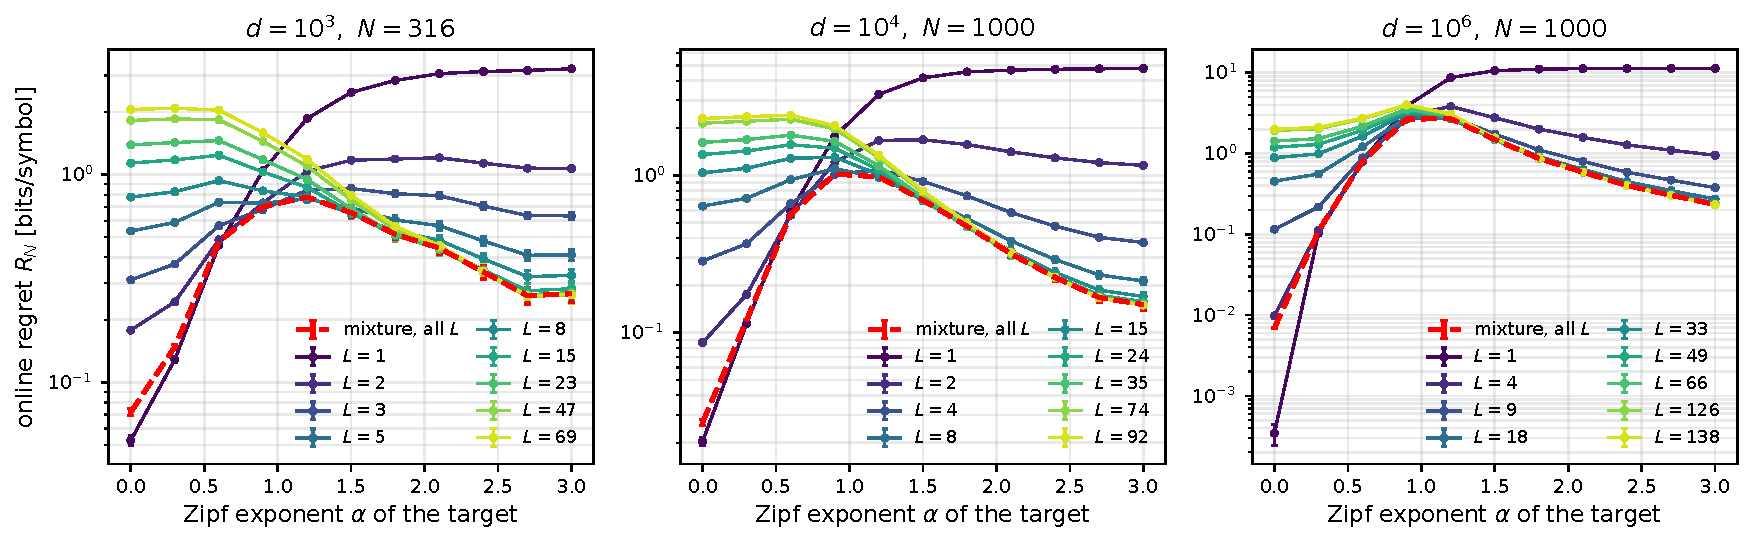
\includegraphics[width=\textwidth]{figures/complexity_spectrum.pdf}
  \caption{Depth tilts the complexity spectrum at every alphabet size.
Online regret on a logarithmic scale versus the Zipf exponent \(\alpha\)
of the target, for \(d=10^3,10^4,10^6\).  Every integer depth up to \(c=L/\ln d\approx10\) was evaluated;
representative depths are displayed for readability.  Shallow priors perform best on near-uniform
targets, while increasingly deep priors perform best as the target becomes
more concentrated.  The dashed red curve is the uniform sequence-mixture
over all depths \(1\le L\le L_{\max}\).
Its gap from the single-depth envelope is bounded by
\((\log_2 L_{\max})/N\) (Remark~\ref{rem:double-mix}); the measured gaps are
reported in the text.
Error bars are profile-sampling standard errors over \(40\) sampled
profiles.}
  \label{fig:spectrum}
\end{figure}
\begin{table}[htp]
  \centering
  \small
  \begin{tabular}{lccccccccccc}
    \toprule
    \(\alpha\) & 0 & 0.3 & 0.6 & 0.9 & 1.2 & 1.5 &
    1.8 & 2.1 & 2.4 & 2.7 & 3.0 \\
    \midrule
    best \(L\) (\(d=10^3\))
      & 1 & 1 & 1 & 3 & 6 & 10 & 15 & 23 & 32 & 43 & 47 \\
    best \(L\) (\(d=10^4\))
      & 1 & 1 & 2 & 4 & 8 & 15 & 24 & 35 & 48 & 63 & 74 \\
    best \(L\) (\(d=10^6\))
      & 1 & 1 & 4 & 9 & 18 & 33 & 49 & 66 & 85 & 110 & 126 \\
    \midrule
    envelope (\(d=10^6\))
      & 0.00 & 0.10 & 0.79 & 2.67 & 2.70 & 1.49 &
        0.87 & 0.59 & 0.40 & 0.30 & 0.23 \\
    \(L{=}1\) (\(d=10^6\))
      & 0.00 & 0.10 & 0.80 & 3.88 & 8.74 & 10.63 &
        11.10 & 11.27 & 11.31 & 11.35 & 11.36 \\
    \bottomrule
  \end{tabular}
  \caption{Best tested depth per target for the three alphabet sizes of
  Figure~\ref{fig:spectrum} (bits/symbol in the last two rows).  Every integer depth up to \(c\lesssim10\) was tested; each entry is
  estimated from \(40\) sampled profiles.  The minimizing
  depth increases broadly with target skew and with \(d\), although the
  regret curves for the more concentrated targets are shallow and therefore
  do not identify the minimizing integer depth sharply.  None of the
  nontrivial minima occurs at the upper search boundary.  }
  \label{tab:spectrum}
\end{table}
Three features of Figure~\ref{fig:spectrum} and Table~\ref{tab:spectrum}
deserve emphasis.
First, the crossing structure is the predicted tilt at every alphabet size.
\(L=1\) is best for the near-uniform targets and performs increasingly
poorly as the target becomes concentrated.  The best tested depth increases
broadly with \(\alpha\) and with \(d\), see Table~\ref{tab:spectrum}.
At \(d=10^6,\alpha=3\), the family envelope improves on
\(L=1\) by a factor of approximately \(49\).
Second, define the \emph{envelope} of the family as the regret of the best
single depth for each target, the pointwise minimum over the curves in
each panel.  The envelope is nearly flat compared with any single member,
and, crucially, it is essentially \emph{achieved} by one predictor: the
depth-average \eqref{eq:depth-average} (dashed red in
Figure~\ref{fig:spectrum}) lies within \((\log_2 L_{\max})/\Nseq\) bits of
the envelope at every \((d,\alpha)\), including \(d=10^6\).
The measured worst-case gaps are $0.01933$, $0.006524$, and $0.006572$ bits
in the three panels, within the corresponding bounds $0.01933$, $0.006524$,
and $0.007109$.  In the first two panels the gap attains the bound exactly:
it occurs on the flattest targets, where the posterior collapses onto
$L=1$, so the average pays the full $\log_2(L_{\max})$ surcharge.  Nothing
is lost beyond the stated price of not knowing the depth in advance.
The family \(\{\model\}_L\), indexed by one integer, has a broad complexity
range in the operational sense of Section~\ref{sec:framework}, and the
range is packaged into a single coherent prior at negligible cost.
\begin{remark}[Why depth-averaging is free]
\label{rem:double-mix}
Computationally, the whole depth family costs no more than its deepest
member: the layer recursion of Appendix~\ref{sec:app-mixture-terms}
computes depth \(L\) from depth \(L-1\), so a single run up to
\(L_{\max}\) produces every depth along the way.  Statistically, the
depth-averaged predictor \eqref{eq:depth-average} pays for its ignorance
of the right depth at most \(\log_2 L_{\max}\) bits \emph{in total} over
the whole sequence, the cost of the uniform \(1/L_{\max}\) factor, i.e.\
at most \((\log_2 L_{\max})/\Nseq\) bits per symbol.  Since the cumulative
regret is the sum over time of the instantaneous prediction errors, the
average tracks the best single depth up to this vanishing overhead, which
is exactly what the dashed curves in Figure~\ref{fig:spectrum} show. 
\end{remark}
Third, the tilt is a statement about the prior, not about fitting: nothing
was trained, and the number of ``parameters'' \(dL\) plays no role in the
crossing: \(L=15\) is \emph{worse} than \(L=1\) on the uniform target despite
being the larger model.  What changes with depth is where the prior
mass sits, i.e.\ which targets are cheap in the sense of
\eqref{eq:prior-mass-bound}.
\section{Scaling Laws from Symbol Discovery}
\label{sec:scaling}
For a Zipf target, the regret is closely tied to the number of
symbols that the sample reveals. Throughout this section, \(R_N\) denotes the normalized online regret
in \eqref{eq:regret-counts}, after \(N\) predictions; thus \(N R_N\)
is the corresponding cumulative online regret. It is computed via
\eqref{eq:regret-profiles}
using the methods described in
Section~\ref{sec:exact-regret}. Let $K_N$ be the number of different
symbols seen in $N$ independent draws from
\begin{equation*}
p_i = \frac{i^{-\alpha}}{H_{d,\alpha}}, \qquad i = 1, \dots, d.
\end{equation*}
Symbol $i$ is seen at least once with probability $1-(1-p_i)^N$.
Hence the expected number of discovered symbols is
\begin{equation}
k_N(d,\alpha) \;:=\; \E[ K_N] \;=\;
\sum_{i=1}^{d}\bigl[1-(1-p_i)^N\bigr].
\label{eq:kN}
\end{equation}
We can compute this sum directly for every $d$, $N$, and $\alpha$
used below.
At logarithmic depth, $L = \mathrm{round}(c \ln d)$, we expect much
of the redundancy to come from identifying the symbols that have
appeared. Saying which $K_N$ of the $d$ symbols were seen takes
$\log_2\binom{d}{K_N}$ bits. This suggests the finite-size law
\begin{equation}
N R_N(d, L, \alpha) \;\approx\;
\E\!\left[\log_2 \binom{d}{K_N}\right]
\;+\; B(c,\alpha)\, k_N .
\label{eq:law}
\end{equation}
The first term is the cost of naming the discovered subset, charged
at one bit of code per bit of description.
The second term charges each discovered symbol a further
$B(c,\alpha)$ bits on top of its share of the description length.
Equation \eqref{eq:law} is
the main finite-size prediction tested in this section. Regret is in
bits throughout, and all logarithms in fits and figures are base 2.
The growth of \eqref{eq:kN} in $N$ can be read off from a simplified
model, reached in three steps: replace $(1-p_i)^N$ by $e^{-N p_i}$,
replace the normalization $H_{d,\alpha}$ of the finite alphabet by the zeta function $\zeta(\alpha)$,
and let the sum run over all $i \ge 1$ rather than stopping at $d$.
\begin{figure}[htp]
  \centering
  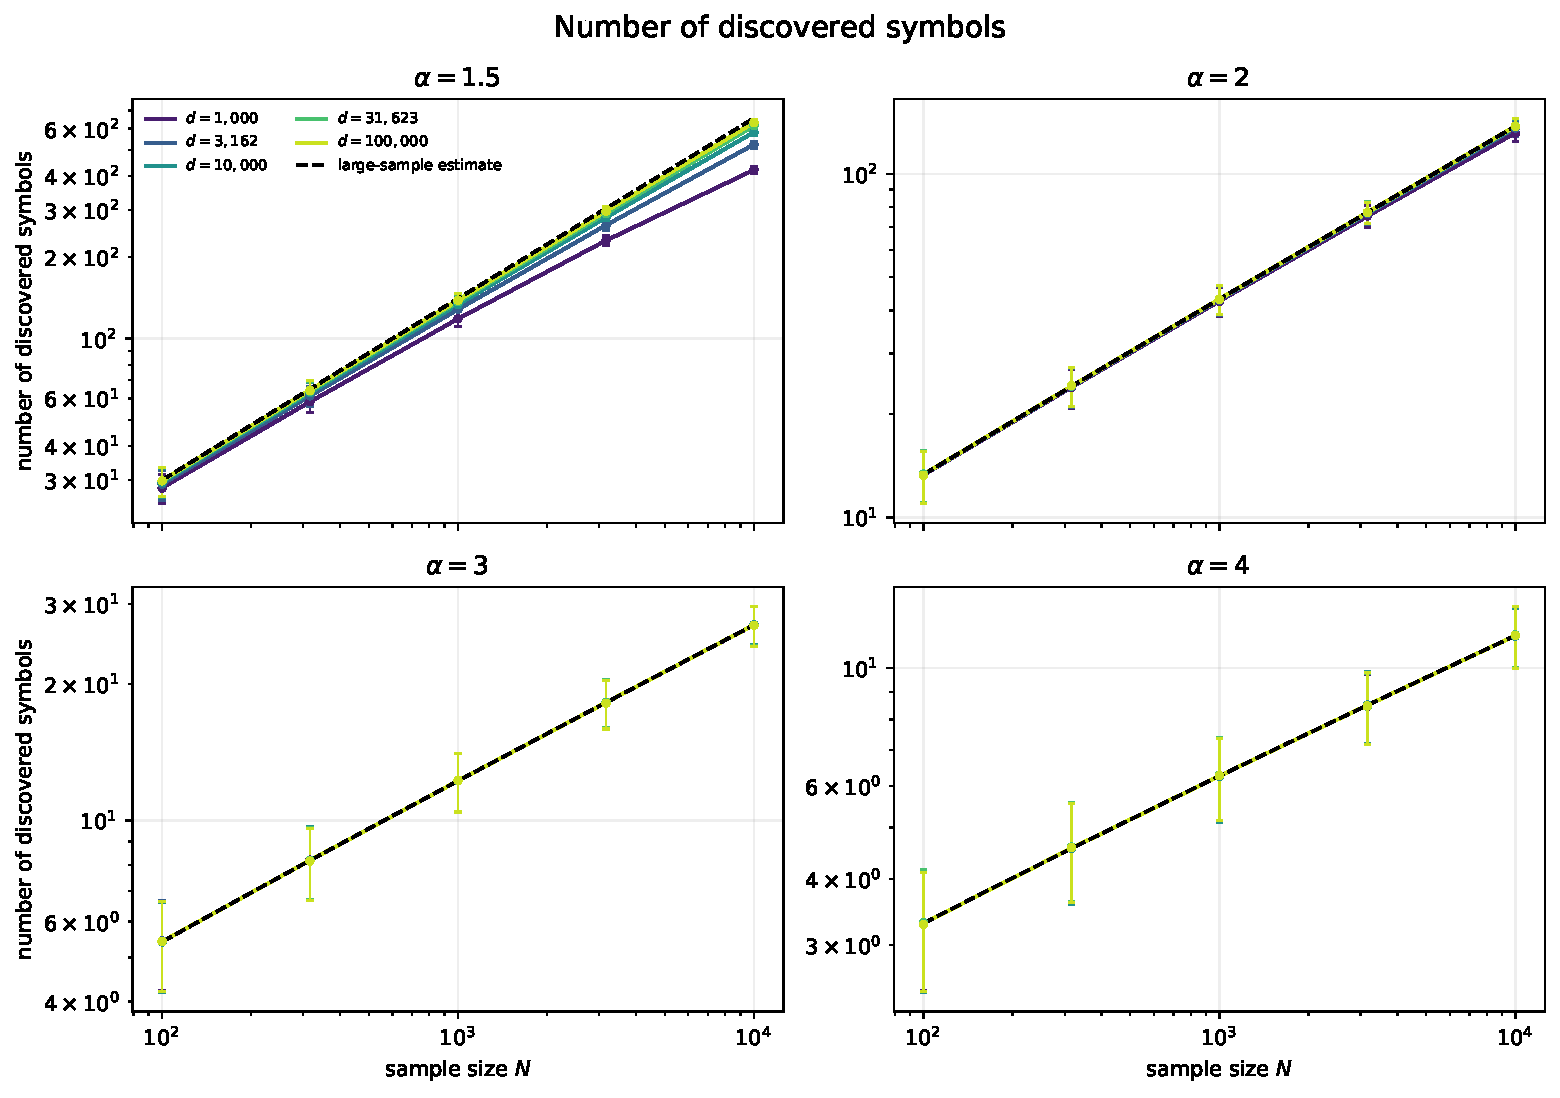
\includegraphics[width=0.92\textwidth]
  {figures/symbol_discovery.pdf}
  \caption{\textbf{Symbol discovery.}
  Solid curves give the exact expected number of discovered symbols,
  dashed curves give the large-sample approximation in
  Equation~\eqref{eq:kN-asym}, and points with error bars give the mean and
  standard deviation over \(5{,}000\) sampled profiles. The effect of the
  finite alphabet is visible mainly at \(\alpha=1.5\) and small \(d\).}
  \label{fig:kN-val}
\end{figure}
Comparing the simplified sum with the integral
$\int_0^\infty \bigl(1-e^{-N x^{-\alpha}/\zeta(\alpha)}\bigr)\,dx$
gives
\begin{equation}
k_N \;=\; \Gamma\!\Bigl(1-\tfrac1\alpha\Bigr)
\Bigl(\tfrac{N}{\zeta(\alpha)}\Bigr)^{1/\alpha}
\;-\; \tfrac12 \;+\; o(1),
\label{eq:kN-asym}
\end{equation}
where the $o(1)$ refers to the simplified model as $N \to \infty$.
The integral equals the first term. The $-\tfrac12$ arises because the sum starts at $i=1$ while the
integral starts at $0$: matching each term of the sum to the unit
interval around it leaves $(0,\tfrac12)$ uncovered, where the
integrand is one.
The cost of the three steps is dominated by the last one: the
infinite sum counts symbols beyond $d$, about
$N d^{1-\alpha}/((\alpha-1)\zeta(\alpha))$ of them, so
\eqref{eq:kN-asym} overshoots \eqref{eq:kN} once the sample starts
to exhaust the alphabet. On the grid of Section~\ref{sec:tests} the
overshoot stays below $5\%$ for $\alpha \ge 2$. At $\alpha = 1.5$ it
grows with the revealed fraction of the alphabet: at $N = 10^4$ it
is $4\%$ of the count at $d = 10^5$ but $55\%$ at $d = 10^3$, where
the sample has revealed $42\%$ of the alphabet. The first two steps
cost at most a few symbols and act in the opposite direction.
Figure~\ref{fig:kN-val} compares \eqref{eq:kN}, \eqref{eq:kN-asym},
and the counts observed in the sampled profiles. All tests below use
the exact count \eqref{eq:kN}; equation~\eqref{eq:kN-asym} serves
only to exhibit the growth $N^{1/\alpha}$.
Substituting \eqref{eq:kN-asym} into \eqref{eq:law} and keeping only
the leading orders gives the simple law
\begin{equation}
R_N(d, L, \alpha) \;\approx\; C(c,\alpha)\,(\log_2 d)\,
N^{-(1-1/\alpha)}.
\label{eq:leading}
\end{equation}
Equation \eqref{eq:leading} is easy to remember, but it stacks
several approximations. At finite $d$ and $N$, we expect
\eqref{eq:law} to be more informative.
\subsection{Three numerical tests}
\label{sec:tests}
We test alphabet size, data, and depth separately. The data and alphabet scaling tests use
\begin{equation*}
N \in \{10^{2},\, 10^{2.5},\, 10^{3},\, 10^{3.5},\, 10^{4}\},
\qquad
d \in \{10^{3},\, 10^{3.5},\, 10^{4},\, 10^{4.5},\, 10^{5}\},
\end{equation*}
with $\alpha \in \{1.5, 2, 3, 4\}$ and $c = \cstar =
(1-\gamma)^{-1}$; the depth test uses $d = 10^{5}$ and $N = 10^{3}$.
At $\alpha = 1.5$ discovery is fastest, with $k_N$ up to about 630;
at $\alpha = 4$ only $k_N \approx 3$ to $12$ symbols are discovered,
so this is where small-count effects show.
\paragraph{Alphabet scaling.}
We first fix $N$, $c$, and $\alpha$, and vary only $d$. Dividing
\eqref{eq:law} by $k_N$ gives
\begin{equation}
\frac{N R_N}{k_N} \;\approx\;
\frac{\E\log_2\binom{d}{K_N}}{k_N} \;+\; B(c,\alpha).
\label{eq:alphabet}
\end{equation}
Write $x$ for the first term on the right of
\eqref{eq:alphabet}, the description length per discovered symbol.
For every $d$, $N$, and $\alpha$, the value of $x$ is a number we
compute, while the left side, $y = N R_N / k_N$, is a number we
measure. Equation \eqref{eq:alphabet} says $y = x + B$. So if we
plot the measured $y$ against the computed $x$, with $d$ moving the
points along the horizontal axis, the points should fall on a
straight line of slope one, lying $B$ above the diagonal. The slope is
the substance of the test: it measures how many bits of code the prior
spends per bit of description. If the prior spent one and a half bits
per bit, the slope would come out $1.5$. The second prediction of
\eqref{eq:alphabet} is that the offset $B$ of the line is the same
for every $N$.
Table~\ref{tab:alphabet} gives the measured slope and offset for three
values of \(N\). For \(\alpha\geq2\), the slopes range from \(0.95\) to
\(1.09\), close to the predicted value one. The agreement is especially
stable at \(\alpha=3\) and \(4\).
The result differs at \(\alpha=1.5\). The measured slope decreases from
\(0.87\) at \(N=10^2\) to \(0.58\) at \(N=10^4\). In this regime the sample
reveals a substantial fraction of the smaller alphabets, so the description
cost is no longer proportional to the expression used in
Equation~\eqref{eq:alphabet}.
The offset slightly changes with \(N\) for every \(\alpha\).
\begin{remark} \label{rem:alpha-part} Part of the growth of $B$ with $\alpha$ has a
simple origin. The target weights fall like $i^{-\alpha}$, so
symbol $i$ carries $(K_N/i)^{\alpha}$ times the weight of the last
discovered symbol, symbol $K_N$. The prior must lift its
coordinate for symbol $i$ by the same factor, which is
$\alpha \log_2 (K_N/i)$ bits, and each bit of lift costs about one
bit of code (derived in the depth test below). Averaged over the
discovered symbols $i \le K_N$, the lift is
$\alpha \log_2\!\bigl(K_N^{K_N}/K_N!\bigr)/K_N
\to \alpha \log_2 e$ bits per discovered symbol, since
$K_N! \approx (K_N/e)^{K_N}$. This matches the direction seen in
Table~\ref{tab:alphabet}: at every $N$, the measured $B$ increases
with $\alpha$.
\end{remark}
\begin{table}[htp]
  \centering
  \begin{tabular}{c l ccc}
    \toprule
    \(\alpha\) & measured quantity
    & \(N=10^2\) & \(N=10^3\) & \(N=10^4\) \\
    \midrule
    \(1.5\) & slope               & \(0.87\) & \(0.76\) & \(0.58\) \\
            & offset \(B\) (bits) & \(-2.74\) & \(-2.17\) & \(-1.34\) \\
    \addlinespace
    \(2\)   & slope               & \(1.00\) & \(0.99\) & \(0.95\) \\
            & offset \(B\) (bits) & \(-0.83\) & \(-0.64\) & \(-0.46\) \\
    \addlinespace
    \(3\)   & slope               & \(1.04\) & \(1.04\) & \(1.04\) \\
            & offset \(B\) (bits) & \(1.40\) & \(1.82\) & \(1.94\) \\
    \addlinespace
    \(4\)   & slope               & \(1.07\) & \(1.09\) & \(1.08\) \\
            & offset \(B\) (bits) & \(2.75\) & \(3.47\) & \(3.90\) \\
    \bottomrule
  \end{tabular}
  \caption{\textbf{Alphabet scaling.}
  For each \(N\), the alphabet size varies from \(10^3\) to \(10^5\).
  Equation~\eqref{eq:alphabet} predicts slope one and an offset \(B\) that
  does not change with \(N\). The table reports both measured quantities.}
  \label{tab:alphabet}
\end{table}
 \paragraph{Data scaling.}
We hold $d$, $c$, and $\alpha$ fixed and vary only $N$. The measured exponent is minus the
slope of a straight line fitted to $\log R_N$ against $\log N$, where $R_N$ is the actual regret.
The right side of the law \eqref{eq:law} predicts how this regret
should scale: the description length of the discovered set, plus
$B$ bits per discovered symbol, divided by $N$.  For $B$ we take a single formula across the whole grid,
$\alpha\log_2 e - 2$ bits: the growth $\alpha\log_2 e$ is that of
Remark~\ref{rem:alpha-part}, and the constant $-2$ was chosen once,
after inspecting the measurements of Table~\ref{tab:alphabet}, to
work across the grid, so the prediction is partly calibrated rather
than fully independent;
moving it by $\pm 0.5$ bits moves the predicted exponents by less
than $0.01$ for $\alpha \ge 2$. The same straight-line fit through
the predicted values gives the predicted exponent.
Table~\ref{tab:data} and Figure~\ref{fig:data} label this
prediction refined and the limit $1 - 1/\alpha$ simple.
Table~\ref{tab:data} compares the slopes. The predicted exponent
differs from the measured one by at most $0.002$ at $\alpha = 2$,
by at most $0.007$ at $\alpha = 3$, and by $0.013$ to $0.019$ at
$\alpha = 4$. The gaps at $\alpha = 3$ and $4$ have an
identifiable origin: the prediction fixes $B$ while
Table~\ref{tab:alphabet} shows it rising slowly with $N$.
Repeating the prediction with the measured $B(\alpha,N)$,
interpolated linearly in $\log N$, shrinks these four gaps to at most
$0.002$. At $\alpha = 1.5$ the prediction is within $0.015$ of the
measurement at $d = 10^5$ and off by $0.10$ at $d = 10^3$; this difference is explained in the last paragraph.
\begin{table}[htp]
  \centering
  \begin{tabular}{c c cc cc}
    \toprule
    & simple & \multicolumn{2}{c}{\(d=10^3\)}
    & \multicolumn{2}{c}{\(d=10^5\)} \\
    \(\alpha\) & prediction & refined & measured & refined & measured \\
    \midrule
    \(1.5\) & \(0.333\) & \(0.619\) & \(0.520\) & \(0.421\) & \(0.436\) \\
    \(2\)   & \(0.500\) & \(0.607\) & \(0.608\) & \(0.544\) & \(0.546\) \\
    \(3\)   & \(0.667\) & \(0.696\) & \(0.689\) & \(0.678\) & \(0.672\) \\
    \(4\)   & \(0.750\) & \(0.754\) & \(0.735\) & \(0.744\) & \(0.731\) \\
    \bottomrule
  \end{tabular}
  \caption{\textbf{Data scaling.}
  Predicted and measured exponents over the tested range
  \(100\leq N\leq10^4\). The simple prediction is \(1-1/\alpha\).
  The refined prediction evaluates the finite-size law on the same values
  of \(N\), with the fixed offset \(B=\alpha\log_2 e-2\) bits per
  discovered symbol; see the text.}
  \label{tab:data}
\end{table}
The limit of the slopes is the discovery rate: by the simple law
\eqref{eq:leading} the slope tends to $1 - 1/\alpha$, the rate at
which the sample reveals new symbols. Over the tested range the
measured slopes sit above this limit at $\alpha = 2$ and $3$ and
below it at $\alpha = 4$. The dominant deviation is the fall of
the regret per discovered symbol $P = N R_N / k_N$. By
\eqref{eq:law} with $\log_2\binom{d}{k} \approx k \log_2(ed/k)$ it
is $P \approx \log_2(ed/k_N) + B$, so each factor of $e$ in $N$
raises $k_N$ by $e^{1/\alpha}$ and lowers $P$ by
$\log_2 e/\alpha$ bits if $B$ does not change, and the slope
becomes
\begin{equation}
\beta_{\mathrm{eff}}
\;=\; 1 - \frac{d\ln k_N}{d\ln N} - \frac{d\ln P}{d\ln N}
\;=\; \Bigl(1 - \tfrac1\alpha\Bigr) + \frac{\log_2 e}{\alpha P}.
\label{eq:beta-eff}
\end{equation}
At \(\alpha=2\), the second term increases from \(0.11\) to \(0.18\)
over the tested range of \(N\) at \(d=10^3\), and from \(0.055\) to
\(0.070\) at \(d=10^5\).  These local corrections are larger than the
fitted excesses \(0.108\) and \(0.046\), because Equation \eqref{eq:beta-eff} omits
two effects that act in the opposite direction: the $-\tfrac12$ of
\eqref{eq:kN-asym} and the rise of $B$ with $N$. At $\alpha = 3$
they cancel about half of the second term; at $\alpha = 4$ they
are as large as it, and the measured slopes land below the limit.
The prediction assumes that the sample reveals a small fraction of
the alphabet. At $\alpha = 1.5$ this holds at $d = 10^5$, where
the predicted and measured slopes are $0.42$ and $0.44$, and fails
at $d = 10^3$, where $N = 10^4$ reveals $42\%$ of the alphabet and
the slopes are $0.62$ predicted against $0.52$ measured.
Figure~\ref{fig:data} shows the comparison at every tested
alphabet size.
\begin{figure}[htp]
  \centering
  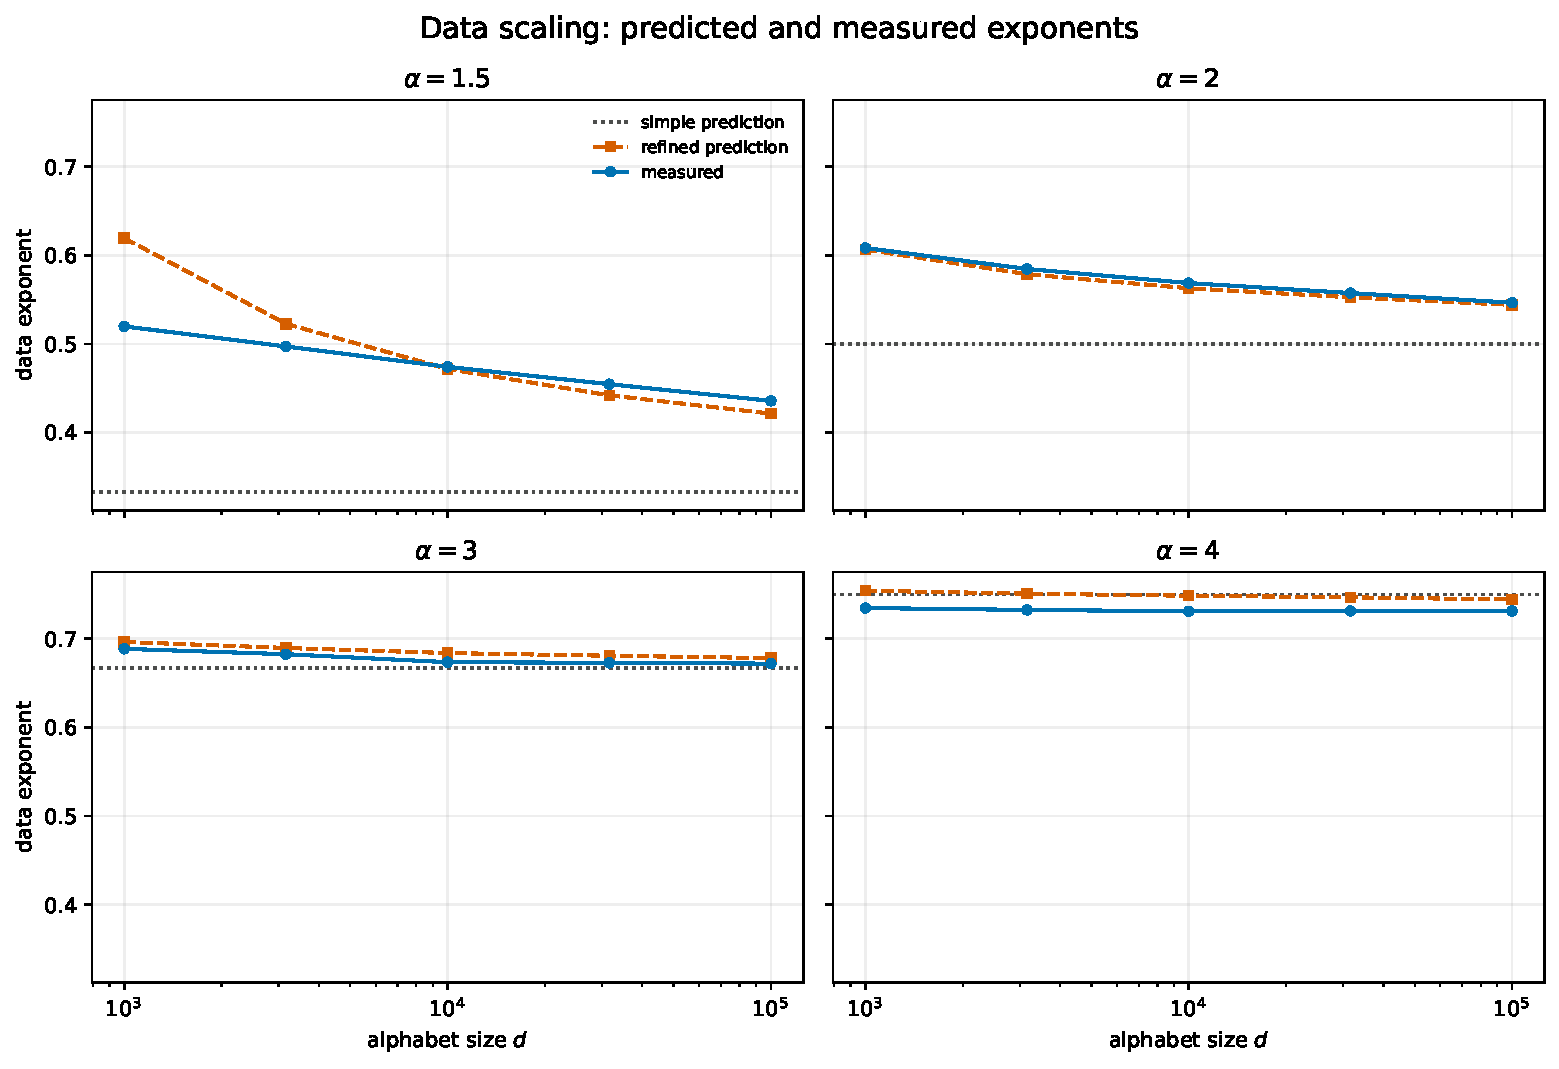
\includegraphics[width=0.92\textwidth]
  {figures/data_scaling.pdf}
  \caption{\textbf{Data scaling.}
  The exponent obtained from the measured regret is compared with the simple
  prediction \(1-1/\alpha\) and with the finite-size prediction evaluated on
  the same values of \(N\). The refined prediction follows the measurements
  closely for \(\alpha=2\) and \(3\). At \(\alpha=1.5\), it fails for the
  smallest alphabet, where the sample reveals a substantial fraction of all
  symbols. At \(\alpha=4\), the measured exponent remains slightly below
  both predictions.}
  \label{fig:data}
\end{figure}
\paragraph{Depth scaling.}
In both tests above, the depth was fixed at $c = \cstar$, and the quantity we worked with was the regret per discovered symbol,
$P = N R_N / k_N$. The third test asks how it depends on the depth: we fix $d = 10^{5}$,
$N = 10^{3}$, and $\alpha$, and vary $c$. Figure~\ref{fig:depth}
shows the result. Shallow depths are clearly worse, while the curves flatten near
\(\cstar\). The best tested depth improves on \(\cstar\) by \(1.2\%\) at
\(\alpha=2\), \(5.9\%\) at \(\alpha=3\), and \(9.5\%\) at \(\alpha=4\);
see Figure~\ref{fig:depth} and Table~\ref{tab:depth}.
Two facts explain this shape. First, the price of naming can never
be below one bit of code per bit of description. The prior treats
all symbols the same, so its weight splits equally over the
$\binom{d}{k}$ possible placements of $k$ discovered symbols, and
any one placement can carry at most a fraction
$\binom{d}{k}^{-1}$ of it: the full description length must always
be paid. Second, whether the prior reaches this floor depends on
where its weight typically sits, and that is what depth controls
(Section~\ref{sec:spectrum}). Past $\cstar$, a typical draw from the prior already
concentrates its mass on a few coordinates. The only information
missing is which coordinates these are, and that is exactly the
description: the price is one, and extra depth cannot lower it.
This is why the curves are flat past $\cstar$, and why the slope
measured in the alphabet test, which runs at $c = \cstar$, comes
out close to one for $\alpha \ge 2$. Below $\cstar$, a typical draw is spread over the whole
simplex. Sparse vectors are then unusual for the prior, and
reaching them costs extra weight on top of the description; each
missing layer makes this surcharge larger.
The surcharge can be computed. A coordinate that carries visible
mass must have its logarithm about $\ln d$ above the typical
level, and this excess must be assembled from the $L = c \ln d$
layers, each contributing $1/c$ on average. The cost for one layer
to shift its logarithm by a given amount is a standard convex
function $\rate$, determined by the distribution of a single
layer factor; for our factors, $\rate$ is the Legendre
transform of $\log\Gamma(1+s)$. The total cost is then $L\,\rate\!\Bigl(\tfrac1c\Bigr)$
against a required shift of $\ln d$, and their ratio is the price
per bit of description:
\begin{equation}
\price(c) \;=\; c\,\rate\!\Bigl(\tfrac1c\Bigr) \quad (c \le \cstar),
\qquad
\price(c) \;=\; 1 \quad (c \ge \cstar).
\label{eq:Ac}
\end{equation}
Because the digamma function satisfies $\psi(2) = 1-\gamma$, three exact facts follow:
$\price(\cstar) = 1$, $\price'(\cstar) = 0$, and
$\price''(\cstar) = (1-\gamma)^3/(\pi^2/6-1) \approx 0.117$. The
price reaches its floor exactly at $\cstar$, and it does so flatly.
On the shallow side, $\price(1) = 1.31$, $\price(1.5) = 1.07$, $\price(2) = 1.01$.
This matches the measurements: the steep rise at small $c$, the
broad minima of Table~\ref{tab:depth}, which are broad because
$\price'(\cstar) = 0$, and the absence of any kink in the regret at the
phase transition, which sits exactly at the flat minimum.
\begin{remark}
The argument behind \eqref{eq:Ac} takes the required growth of a
coordinate to be exactly a factor of $d$, and it ignores how the
typical size of all the other coordinates shifts with depth. It is
therefore reliable near and above $\cstar$ and overshoots for
$c \lesssim 1$. A full derivation through the induced density of
Section~\ref{sec:spectrum} is open; it would also give the dependence
of the offset $B$ on $N$, and the phase structure it needs is that of
\cite{jeong2026phase}.
\end{remark}
\begin{figure}[htp]
  \centering
  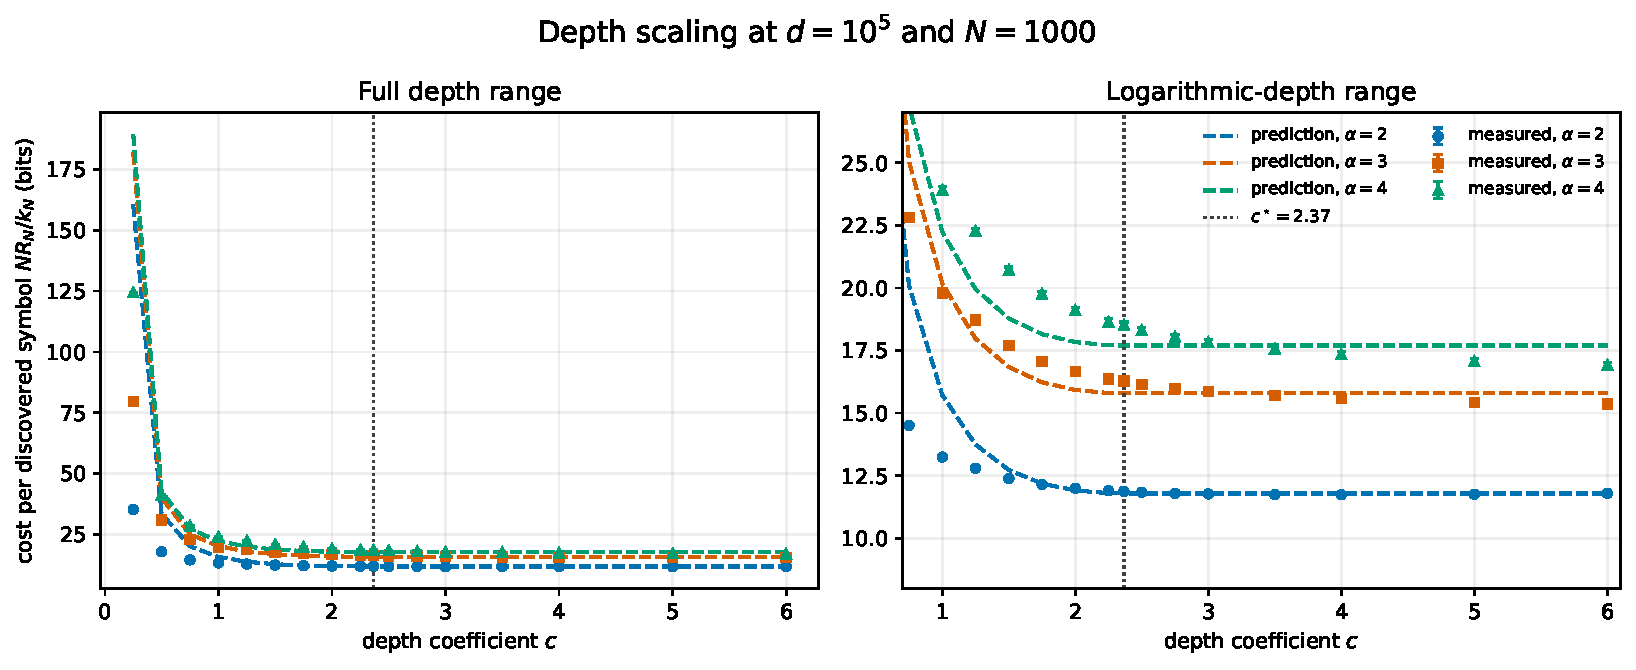
\includegraphics[width=0.98\textwidth]
  {figures/depth_scaling.pdf}
  \caption{\textbf{Depth scaling.}
  Measured regret per discovered symbol at \(d=10^5\) and \(N=10^3\),
  together with the prediction in Equation~\eqref{eq:Ac}. The left panel
  shows the full range. The right panel enlarges the logarithmic-depth
  range. The prediction captures the broad flattening near \(\cstar\), but
  overestimates it at the shallowest depths, as expected from the
  approximation used to derive it.}
  \label{fig:depth}
\end{figure}
\begin{table}[t]
  \centering
  \begin{tabular}{ccc}
    \toprule
    \(\alpha\) & best tested \(c\) & \(P(\cstar)/P_{\min}\) \\
    \midrule
    \(2\) & \(4\) & \(1.012\) \\
    \(3\) & \(6\) & \(1.059\) \\
    \(4\) & \(6\) & \(1.095\) \\
    \bottomrule
  \end{tabular}
  \caption{\textbf{Depth scaling.}
  Measured dependence of the regret per discovered symbol on depth at
  \(d=10^5\) and \(N=10^3\).}
  \label{tab:depth}
\end{table}
\paragraph{Conclusion.}
The three experiments support a common account of the regret. After
$N$ samples, about $k_N$ symbols have been seen. Saying which ones
takes $\log_2\binom{d}{k_N}$ bits, and as long as the sample
reveals only a small fraction of the alphabet, the prior pays this
in full and not more: for $\alpha \ge 2$ the measured slopes are close to
one (Table~\ref{tab:alphabet}), and the depth test derives the value one
at $c = \cstar$.
At $\alpha = 1.5$ the smallest
alphabets leave this regime, and the description term is no longer
the right measure of the naming cost. Each discovered symbol costs a
further $B$ bits, where $B$ grows with the concentration of the
target (Remark~\ref{rem:alpha-part}) and drifts slowly with $N$; we
report it rather than model it. Together, the finite-size law \eqref{eq:law} and its leading form
\eqref{eq:leading} summarize the account: the exponent is the rate of
symbol discovery, and depth, once logarithmic, moves only the constants,
in the way \eqref{eq:Ac} states.

\section{Competitive Comparison: Classical, Good--Turing, Ristad, and the LSA
Predictor}
\label{sec:comparison}
The scaling analysis says the log-depth prior handles heavy-tailed targets on
large alphabets well.  The natural external benchmark is the line of work on
competitive distribution estimation, where Good--Turing-type estimators are
provably near-oracle \cite{orlitsky2015competitive,acharya2013tight,
orlitsky2003always,mcallester2000leave}.  This section uses the LSA prior on the experimental suite of Orlitsky and Suresh
\cite{orlitsky2015competitive} and adds Ristad's natural law of succession
\cite{ristad1995natural}, which we argue is the closest classical relative of
the LSA prior.
\subsection{Setup}
\label{sec:comparison-setup}
Following \cite{orlitsky2015competitive}, the support size is \(d=10^4\).
Their six targets are used: uniform; a step distribution with half the
symbols of probability \(\tfrac1{2d}\) and half \(\tfrac3{2d}\); Zipf with
\(\alpha=1\) and \(\alpha=1.5\); and random targets drawn once per trial
from the Dirichlet-\(1\) and Dirichlet-\(\tfrac12\) priors on
\(\Delta_d\), together with five additional targets that widen the range
of shapes: Zipf with \(\alpha=2\), \(3\), \(4\), and \(5\) (increasingly
concentrated; at \(\alpha=5\) the top symbol carries \(96\%\) of the mass
and its count approaches \(2\cdot10^4\) at the largest sample size,
handled by the heavy-count extension of
Appendix~\ref{sec:app-anchors}); and a geometric
law \(p_i\propto0.998^{\,i}\), whose probabilities decay exponentially
over an effective support of about \(500\) symbols.
For each target and each
\(n\in\{1000,2000,3000,5000,7000,10^4,1.4\cdot10^4,2\cdot10^4\}\), a sample
of size \(n\) is drawn, every estimator is given the resulting counts
\((m_1,\dots,m_d)\) (and the support size \(d\)), and the loss is the
divergence \(\KL(p\,\|\,\hat q)\) between the true distribution and the
estimate, averaged over \(20\) independent trials with common samples across
estimators.  For a Bayesian mixture this estimate is the predictive
distribution \(\hat q(i)=Q(x_{n+1}=i\mid x^n)\), so the metric is the
instantaneous form of the cumulative regret studied above: the per-symbol
online regret is exactly the time average of these predictive divergences.
The estimators are:
\begin{itemize}
\item \emph{Add-constant rules}: add-one (Laplace), which by
  Proposition~\ref{prop:laplace} is the prior induced by the LSA at \(L=1\);
  add-half (Krichevsky--Trofimov \cite{krichevsky1981performance}); and the
  Braess--Sauer rule \cite{braess2004bernstein}, which adds
  \(\tfrac12\) to unseen, \(1\) to once-seen, and \(\tfrac34\) to
  multiply-seen symbols before normalizing.
\item \emph{Good--Turing + empirical}: the hybrid of
  \cite{orlitsky2015competitive}: with \(c_t\) the number of symbols
  appearing \(t\) times, a symbol seen \(t\) times receives (before
  normalization) the empirical mass \(t/n\) if \(t>c_{t+1}\), and the
  Good--Turing mass \((c_{t+1}+1)(t+1)/(n\,c_t)\) otherwise;
  unseen symbols share the \(t=0\) assignment.
\item \emph{Ristad's natural law of succession} \cite{ristad1995natural}:
  with \(s\le d\) distinct symbols observed in \(n\) samples, if \(s=d\) the
  rule is add-one; if \(s<d\),
  \[
    \hat q(i)=
    \begin{cases}
      \dfrac{(m_i+1)(n+1-s)}{n^2+n+2s}, & m_i>0,\\[1.2ex]
      \dfrac{s(s+1)}{(d-s)\,(n^2+n+2s)}, & m_i=0 .
    \end{cases}
  \]
  The rule arises from a hierarchical uniform prior over the size and
  identity of the support followed by a uniform Dirichlet within it.
  However, for this rule, as noted in \cite{hutter2014}, the code, or the prediction it implies for the entire sequence does not induce a predictive probability of any prior: its sequence
probability is order-dependent (see discussion in Section~\ref{sec:comparison-findings} and Section~\ref{sec:bible}).
\item \emph{Natural oracle}: the genie of \cite{orlitsky2015competitive}
  that knows \(p\) but must assign the same probability to all symbols with
  the same count: \(\hat q(i)=S_{m_i}/c_{m_i}\), with \(S_t\) the true
  total probability of symbols appearing \(t\) times.  It lower-bounds every
  natural (count-based) estimator, including all of the above.
\item \emph{The prior induced by the LSA} at \(L=5\) and
  \(L=22=\operatorname{round}(c^\star\ln d)\), computed exactly from the
  count profile by the methods of Appendix~\ref{sec:app-mixture-terms}.
\item \emph{Depth-averaged LSA predictor}
  \eqref{eq:depth-average} with \(L_{\max}=80\), comfortably above \(2c^\star\ln d\approx 44\), so
that the most concentrated targets cannot be limited by the ceiling (the
effect of the ceiling is examined in the findings below).  After
observing
  \(x^n\), its next-symbol estimate is the weighted average
  \[
    \hat q(i)
    =
    \sum_{L=1}^{80} w_L(x^n)\,\hat q_L(i),
    \qquad
    w_L(x^n)
    =
    \frac{Q^{(L)}_n(x^n)}{\sum_{L'=1}^{80} Q^{(L')}_n(x^n)},
  \]
  where \(\hat q_L\) is the depth-\(L\) predictive and the weight
  \(w_L\) is the (posterior) probability of depth \(L\) given the data.
  The weights require the mixture likelihoods \(Q^{(L)}_n(x^n)\)
  themselves, not just ratios; these are computed to about \(10^{-3}\)
  nats by the exact-evaluation method of
  Appendix~\ref{sec:app-exact-rows}.
\end{itemize}
\begin{figure}[t]
  \centering
  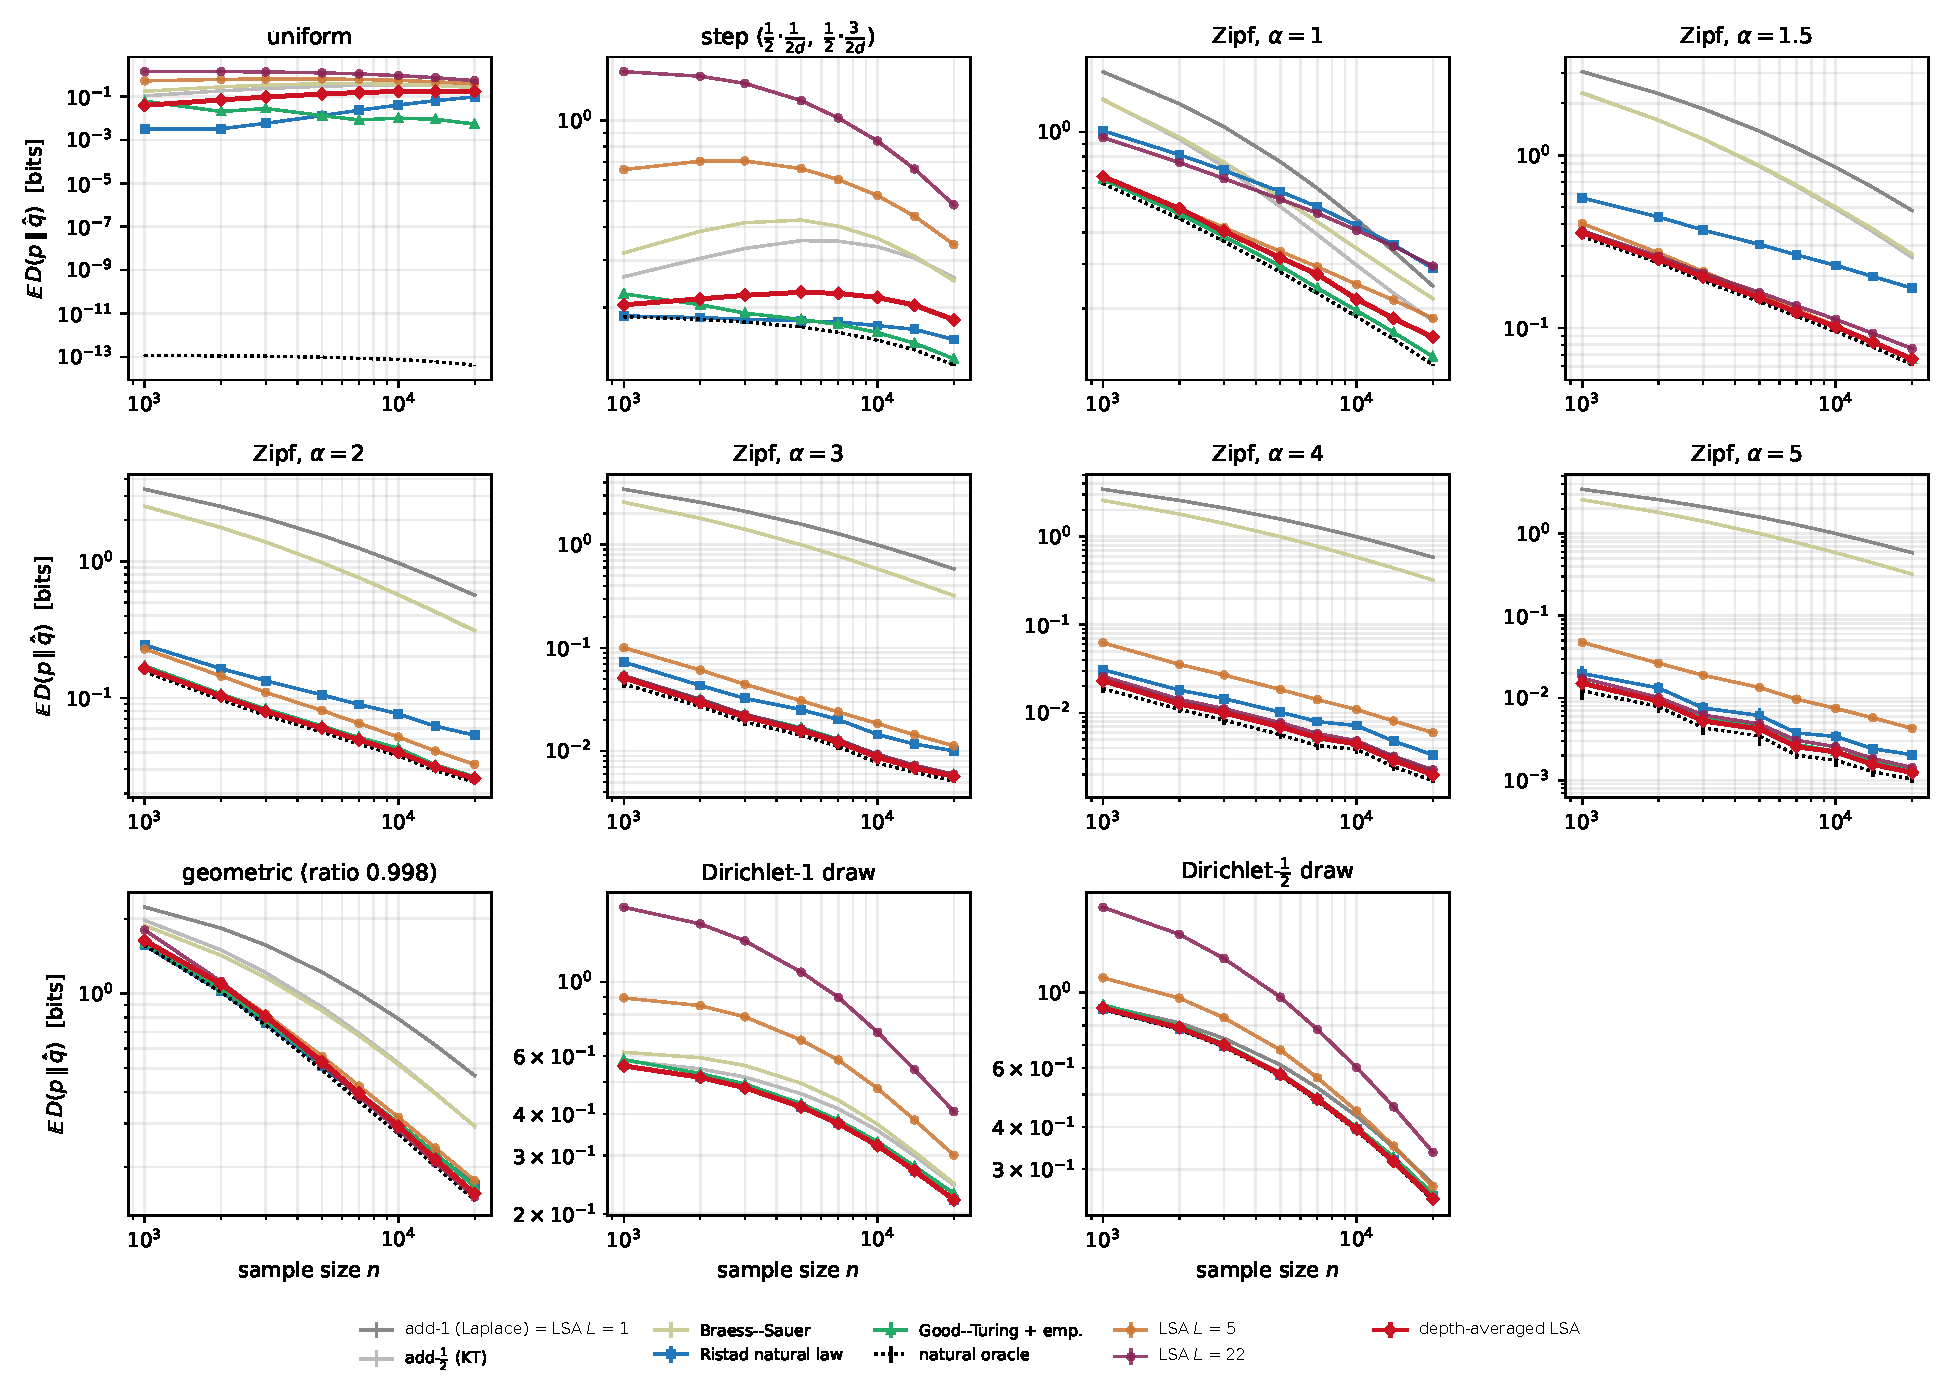
\includegraphics[width=\textwidth]{figures/orlitsky_comparison.pdf}
\caption{Competitive comparison on the benchmark of
\cite{orlitsky2015competitive}, extended to eleven targets
(\(d=10^4\); log-log axes; \(20\) trials, standard-error bars).
The depth-averaged LSA predictor (red diamonds) performs well on
\emph{every} panel: it matches the best add-constant rule on the flat
targets and the best overall rule on eight of eleven panels. On the
uniform target, where it lags behind Good--Turing and Ristad, all
predictors are far from the natural-oracle curve, which is
\(\approx0\).}

  \label{fig:orlitsky}
\end{figure}
\begin{table}[t]
  \centering
  \small
  \setlength{\tabcolsep}{4.5pt}
  \begin{tabular}{lcccccc|ccc}
    \toprule
    & \multicolumn{6}{c|}{classical} & \multicolumn{3}{c}{LSA}\\
    target & add-1 & KT & BS & Ristad & GT & oracle & \(L{=}5\) & \(L{=}22\) & avg over \(L\)\\
    \midrule
    uniform            & 0.174 & 0.285 & 0.262 & 0.098 & 0.005 & 0.000 & 0.387 & 0.544 & 0.174\\
    step               & 0.180 & 0.258 & 0.252 & 0.152 & 0.129 & 0.122 & 0.344 & 0.484 & 0.180\\
    Zipf \(\alpha=1\)  & 0.246 & 0.179 & 0.219 & 0.288 & 0.129 & 0.120 & 0.183 & 0.295 & 0.154\\
    Zipf \(\alpha=1.5\)& 0.479 & 0.257 & 0.268 & 0.170 & 0.066 & 0.061 & 0.066 & 0.076 & \textbf{0.066}\\
    Zipf \(\alpha=2\)  & 0.564 & 0.310 & 0.311 & 0.053 & 0.027 & 0.024 & 0.033 & 0.026 & \textbf{0.026}\\
    Zipf \(\alpha=3\)  & 0.582 & 0.321 & 0.321 & 0.0101 & 0.0059 & 0.0051 & 0.0112 & 0.0060 & \textbf{0.0057}\\
    Zipf \(\alpha=4\)  & 0.584 & 0.322 & 0.322 & 0.0033 & 0.0022 & 0.0017 & 0.0060 & 0.0023 & \textbf{0.0020}\\
    Zipf \(\alpha=5\)  & 0.584 & 0.322 & 0.322 & 0.0020 & 0.0013 & 0.0010 & 0.0043 & 0.0014 & \textbf{0.0012}\\
    geometric          & 0.467 & 0.292 & 0.292 & 0.170 & 0.167 & 0.147 & 0.177 & 0.152 & \textbf{0.156}\\
    Dirichlet-1 draw   & 0.221 & 0.244 & 0.247 & 0.221 & 0.230 & 0.220 & 0.301 & 0.407 & \textbf{0.221}\\
    Dirichlet-\(\tfrac12\) draw & 0.272 & 0.244 & 0.249 & 0.250 & 0.254 & 0.243 & 0.267 & 0.337 & \textbf{0.246}\\
    \bottomrule
  \end{tabular}
  \caption{Mean \(\KL(p\|\hat q)\) in bits at \(n=2\cdot10^4\), \(d=10^4\),
  \(20\) trials; standard errors \(\le0.001\) bits except the Dirichlet
  rows (\(\le0.013\)).  The last column is the depth-averaged LSA predictor
  \eqref{eq:depth-average} over all depths \(L=1,\dots,80\) (see the text), a \emph{single} prior
  with no tuned constants.
Bold marks rows where it beats every classical (non-LSA) method or ties
the best of them within one standard error;
Section~\ref{sec:comparison-findings} discusses the pattern row by row.
  }
  \label{tab:orlitsky}
\end{table}
\begin{table}[t]
  \centering
  \small
  \begin{tabular}{lll}
    \toprule
    target & posterior over depths at \(n=10^3\) & at \(n=2\cdot10^4\)\\
    \midrule
    uniform & \(L{=}1:1.00\) & \(L{=}1:1.00\)\\
    step & \(L{=}1:1.00\) & \(L{=}1:1.00\)\\
    Zipf \(\alpha=1\) & \(L{=}5:0.71,\ L{=}6:0.29\) & \(L{=}3:1.00\)\\
    Zipf \(\alpha=1.5\) & \(L{=}15:0.20,\ L{=}14:0.19,\ L{=}16:0.16,\ L{=}13:0.13\) & \(L{=}9:0.63,\ L{=}10:0.36\)\\
    Zipf \(\alpha=2\) & \(L{=}31,30,32:0.06\) each (broad, \(L\approx26\) to \(36\)) & \(L{=}24,23,25:{\approx}0.15\) each\\
    Zipf \(\alpha=3\) & broad: \(94\%\) of mass on \(L\in[41,80]\) & broad, mode \(L{\approx}70\); \(99\%\) on \(L\in[41,80]\)\\
    Zipf \(\alpha=4\) & broad: \(96\%\) on \(L\in[41,80]\) & \(85\%\) on \(L\in[61,80]\), top weight \(0.07\)\\
    Zipf \(\alpha=5\) & broad: \(96\%\) on \(L\in[41,80]\) & \(86\%\) on \(L\in[61,80]\), top weight \(0.07\)\\
    geometric & \(L{=}4:0.73,\ L{=}5:0.27\) & \(L{=}10:0.92,\ L{=}9:0.08\)\\
    Dirichlet-1 & \(L{=}1:1.00\) & \(L{=}1:1.00\)\\
    Dirichlet-\(\tfrac12\) & \(L{=}2:0.70,\ L{=}1:0.30\) & \(L{=}2:1.00\)\\
    \bottomrule
  \end{tabular}
  \caption{Mean posterior weights \(w_L\propto q_L(x^n)\) of the
depth-averaged predictor (entries below \(0.05\) omitted). The data
select depth as the complexity-spectrum analysis predicts: shallow for
flat targets, deep for heavy-tailed ones.}
  \label{tab:posteriors}
\end{table}
\subsection{Findings}
\label{sec:comparison-findings}
The short summary is that the scheme does well: the depth-averaged
LSA predictor, which is Bayesian and has all the theoretical and practical advantages of a Bayesian, with the layer-induced prior, beats every classical method, or ties the best of them within
one standard error, on eight of the eleven targets; the exceptions, all in
favor of Good--Turing, are the flattest targets (uniform, step, and Zipf
\(\alpha=1\)), and the uniform case, where the gap is largest and most
instructive, is discussed at the end of this section.
The paragraphs below go through the evidence, and
Section~\ref{sec:bible} takes the same estimators to a real text.
\paragraph{On heavy-tailed targets, the LSA prior is
Good--Turing-competitive.}
On Zipf \(\alpha=1.5\), the most skewed Zipf target in the original
benchmark of \cite{orlitsky2015competitive}, the \(L=5\)
mixture attains \(0.066\) bits at \(n=2\cdot10^4\), equal to Good--Turing
(\(0.066\)) and within about \(8\%\) of the natural oracle (\(0.061\));
at \(n=1000\) the deeper members are slightly \emph{ahead} of Good--Turing.
Fixed depths beat Ristad (\(0.170\) at \(n=2\cdot10^4\)) by more than a
factor of two and the add-constant rules by factors of \(3\) to \(7\). On
Zipf \(\alpha=1\), the depth-averaged predictor (\(0.154\)) is second only to
Good--Turing (\(0.129\)), ahead of every other estimator 
and far ahead of Ristad (\(0.288\)) and
add-one (\(0.246\)).  No component of these mixtures was designed around
count frequencies; the competitive behavior emerges from where logarithmic
depth places prior mass.
\paragraph{On strongly concentrated targets the average overtakes
Good--Turing.}
The concentrated targets sharpen the picture.  On Zipf \(\alpha=2\) the
depth-averaged predictor attains \(0.165\) bits at \(n=10^3\) and
\(0.026\) at \(n=2\cdot10^4\), ahead of Good--Turing (\(0.172\) and
\(0.027\)) at both sample sizes and within about \(6\) to \(8\%\) of the natural
oracle; on Zipf \(\alpha=3\) it attains \(0.0057\) versus Good--Turing's
\(0.0059\), close to the oracle (\(0.0051\)); on Zipf \(\alpha=4\)
it reaches \(0.0020\) bits at \(n=2\cdot10^4\) versus Good--Turing's
\(0.0022\), near the oracle (\(0.0017\)); and on Zipf \(\alpha=5\) it
attains \(0.0012\) against Good--Turing's \(0.0013\) and the oracle's
\(0.0010\), the differences at the scale of one standard error
(\(0.0001\)).  The add-constant rules remain \(2\) to \(3.5\)
bits away at small \(n\) on all of these.  
\paragraph{The posterior weights tell the
architectural story.} It is interesting to examine the posterior weights of the depths, up to
\(L_{\max}=80\), which is roughly \(3.7\,c^\star\ln d\).  On \(\alpha=2\) the data
select a band around \(L\approx23\) to \(25\), just beyond
\(c^\star\ln d \approx 22\).  On \(\alpha=3\), \(4\), and \(5\), 
the posterior spreads almost
flat over the deep end (for \(\alpha=4,5\), \(85\)--\(86\%\) of the mass on
\(L\in[61,80]\) with top weight only \(0.07\)), while the regret is
unchanged to the fourth decimal.
Depth beyond roughly \(2c^\star\ln d\) neither helps nor hurts.  This
is the freezing transition of Section~\ref{sec:scaling}, now visible
in the likelihood itself: past \(c^\star\) the price of naming a
discovered symbol, \(\price(c)\) of Equation~\eqref{eq:Ac}, equals one no
matter how deep the prior, so all sufficiently deep members of the
family predict alike and the data cannot tell them apart.




\paragraph{Choosing \(L_{\max}\).}
The experiments above settle a practical question: how deep should the
family be? The evidence converges on
\(L_{\max}=\lfloor 2c^\star\ln d\rceil\approx 3.3\log_2 d\), about three
layers per bit of alphabet (\(44\) at \(d=10^4\), \(65\) at \(10^6\)); the
factor of two over \(c^\star\ln d\) is margin for the finite-\(d\)
crossover, and even the most concentrated target tested gains nothing
beyond it. The two provisioning errors are sharply asymmetric: too small
a ceiling costs real bits on concentrated targets, while too large a
ceiling costs \(\log_2\) of the overshoot factor in total, one bit here
for doubling, with every flat-target row unchanged to three decimals.
When in doubt, round up; the only genuine cost of a generous ceiling is
computation, which grows linearly in \(L_{\max}\).


\paragraph{The geometric target.}
The geometric target rewards moderate depth: the posterior settles at
\(L\approx10\), and the depth-average (\(0.156\) bits at
\(n=2\cdot10^4\)) is ahead of Good--Turing
(\(0.167\)) and Ristad (\(0.170\)).  
Here the fixed depth $L=22$ is slightly better (\(0.152\)), but the
depth-average is close behind while remaining universal.
The target’s exponential decay is neither flat
nor power-law, and no single classical rule is tuned for it; the average
finds the right amount of prior sparsity by itself.
\paragraph{The price appears exactly where the theory says it should.}
On the uniform and step targets, and on the Dirichlet draws (which are
flat targets with \(\Theta(1/d)\) coordinates), the deep priors pay:
\(L=22\) is the worst estimator on the uniform panel (\(0.544\) bits at
\(n=2\cdot10^4\)) while the family’s shallow end, add-one \(=L{=}1\), is
second only to Ristad among the non-GT rules (\(0.174\)).  This is the spectrum tilt
of Section~\ref{sec:spectrum} evaluated on external benchmarks: a deep prior
is not uniformly better; it reallocates regret from skewed to flat targets.
Good--Turing, by contrast, adapts its effective smoothing to the count
statistics and is near-oracle on every panel; this is precisely the content
of its competitive guarantees \cite{orlitsky2015competitive}.

\paragraph{The depth-averaged predictor: one prior, best of the family,
empirically.}
Remark~\ref{rem:double-mix} promises that averaging over all depths incurs essentially no penality relative to the best depth. The ‘‘avg over \(L\)’’
column of Table~\ref{tab:orlitsky} and the red curve of
Figure~\ref{fig:orlitsky} verify the promise on external benchmarks. The
posterior weights (Table~\ref{tab:posteriors}) collapse onto \(L=1\) on
the flat targets, making the average \emph{exactly} add-one there, and
select intermediate depths on the skewed ones; the row-by-row numbers are
in Table~\ref{tab:orlitsky}. Two facts are new here. First, on Zipf
\(\alpha=1.5\) the average is \emph{ahead} of Good--Turing at every
\(n\le1.4\cdot10^4\) (e.g.\ \(0.356\) vs.\ \(0.366\) at \(n=10^3\)).
Second, the posterior adapts: the selected depth \emph{decreases} from
about \(15\) to about \(9\) as \(n\) grows; once the data pin down the
heavy symbols, less prior sparsity is required, and the average
reallocates automatically.

\paragraph{Coherence: what the mixture buys that Good--Turing does not.}
The Good--Turing hybrid is an excellent estimator but not a coherent
probability assignment over sequences: its post-hoc normalization and
regime switch (empirical vs.\ Good--Turing mass) do not arise from any prior,
and its cumulative log-loss admits no mixture interpretation.  The
depth-averaged LSA predictor is a single exchangeable prior: it
simultaneously defines a sequential code, satisfies the regret identity
\eqref{eq:regret-profiles}, composes with further hierarchical modeling,
and inherits the non-uniform guarantee \eqref{eq:prior-mass-bound}.  The
comparison shows that this coherence is now essentially free: across the
whole benchmark, the coherent prior gives up meaningful ground to
Good--Turing only on the uniform target.  There Good--Turing exploits a
piece of information this prior family does not use, the observed
frequencies of the counts themselves, which on a uniform target reveal
that all symbols have nearly the same probability, and it reaches
\(0.005\) bits where the best prior in the family reaches \(0.174\).

\paragraph{Ristad's law as the closest relative.}
Ristad’s natural law is built from a two-level hierarchical picture, mass
spread first over support sizes and then uniformly within a support
\cite{ristad1995natural}, and its qualitative behavior in
Figure~\ref{fig:orlitsky} sits between the add-constant rules and
Good--Turing, much like a two-level layered prior. 
Furthermore, as noted above,
unlike the LSA predictors, Ristad's law is not exactly Bayesian:
It was derived combinatorially, and its one-step rules do not multiply
to an exchangeable probability over sequences \cite{hutter2014} (already at \(d=2\),
sequences with the same counts receive different probabilities). Ristad's sequential version is also the one used in the next 
Section~\ref{sec:bible}, to encode the entire sequence (the Bible).

Concretely, as for its performance: on Zipf \(\alpha=1.5\), Ristad improves on add-one by
\(2.8\times\) and the log-depth mixture improves on Ristad by a further
\(2.6\times\), closing essentially all the remaining gap to the oracle.
Where Ristad's two-level prior is better adapted (near-uniform targets:
\(0.098\) vs.\ Laplace's \(0.174\) on uniform), the deep prior has moved its
mass elsewhere.
\subsection{Compressing the Bible}
\label{sec:bible}
The benchmark above scores estimators against known synthetic targets.  As
a final test we compress a real text and measure each estimator by its
actual codelength.  The corpus is the entire King James Bible (Project
Gutenberg etext \#10, verse numbers removed): \(N=915{,}860\) tokens over
a fixed vocabulary of \(d=100{,}000\), the alphabet scale of modern language-model tokenizers, of which the text uses
\(13{,}550\) distinct word and punctuation types, about \(14\%\) of the
alphabet.  Every estimator is a sequential probability assignment, hence a
lossless code: its codelength is \(-\log_2\) of the probability it assigns
to the token sequence.  We report the \emph{redundancy}: codelength per
token minus the empirical unigram entropy \(\hat H_n\) of the coded prefix, the part of the codelength due to \emph{learning} the distribution
rather than to its intrinsic uncertainty.  For the exchangeable estimators
(the LSA priors, add-one, add-half) the codelength is
computed exactly from the counts; for the order-dependent rules
(Good--Turing, Ristad, Braess--Sauer) it is accumulated by coding the
actual sequence one token at a time.
Each number reported in this section is the codelength of an honest
sequential predictor: predict the next token, suffer the log-loss, update,
repeat.  Appendix~\ref{sec:app-validation} states the identity between the
batch codelength and the accumulated sequential log-loss, and verifies it
numerically on the corpus.

\begin{table}[t]
  \centering
  \small
  \begin{tabular}{rrcccccccc}
    \toprule
    \(n\) & distinct & \(\hat H_n\) & add-1 & KT & BS & Ristad & GT &
    LSA avg & posterior mode\\
    \midrule
    \(10{,}000\)  & 1{,}160  & 7.56 & 4.597 & 3.846 & 3.805 & 1.193 & 1.066 & \textbf{1.052} & \(L=21\)\\
    \(30{,}000\)  & 2{,}119  & 7.87 & 3.225 & 2.512 & 2.489 & 0.709 & 0.606 & \textbf{0.598} & \(L=21\)\\
    \(100{,}000\) & 3{,}839  & 8.02 & 1.911 & 1.359 & 1.350 & 0.381 & 0.310 & \textbf{0.306} & \(L=21\)\\
    \(300{,}000\) & 6{,}922  & 8.18 & 1.026 & 0.679 & 0.677 & 0.224 & 0.170 & \textbf{0.168} & \(L=19\)\\
    \(915{,}860\) & 13{,}550 & 8.48 & 0.478 & 0.303 & 0.302 & 0.137 & 0.097 & \textbf{0.095} & \(L=15\)\\
    \bottomrule
  \end{tabular}
  \caption{Compressing the King James Bible (\(d=100{,}000\),
  word-and-punctuation tokens).  Redundancy in bits per token (codelength
  per token minus the empirical unigram entropy \(\hat H_n\)) for prefixes
  of \(n\) tokens.  The depth-averaged LSA predictor is the
  best method at every prefix length; its posterior over depths is
  essentially a point mass that drifts from \(L=21\) down to \(L=15\) as
  the sample grows.}
  \label{tab:bible}
\end{table}
\begin{figure}[t]
  \centering  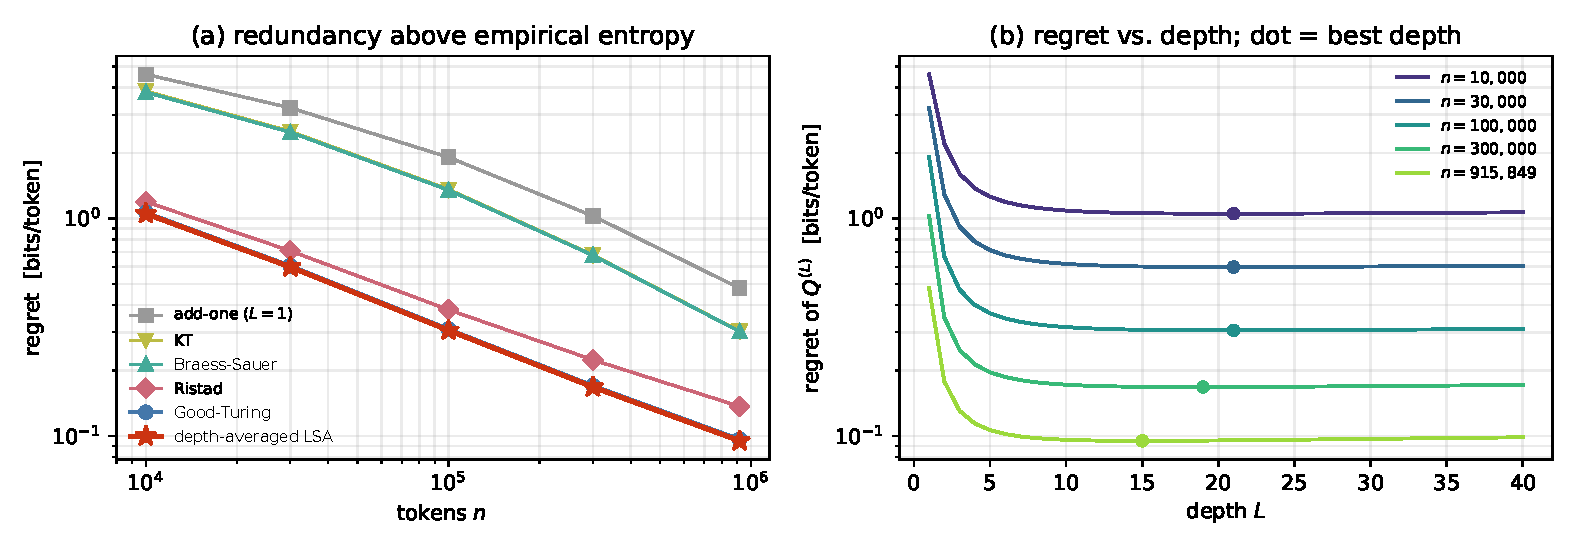
\includegraphics[width=\textwidth]{figures/bible_full.pdf}
  \caption{The Bible experiment.  (a)~Redundancy above the empirical
  entropy for each method as the coded prefix grows (log-log); the
  depth-averaged LSA predictor (red) is lowest at every
  \(n\).  (b)~Redundancy of the single-depth mixtures \(Q^{(L)}\) as a
  function of depth, at each prefix length; the minimizing depth (dots)
  moves from \(L=21\) to \(L=15\) as \(n\) grows, and the depth-average
  matches the minimum to four decimal places throughout.}
  \label{fig:bible}
\end{figure}
Table~\ref{tab:bible} and Figure~\ref{fig:bible} show the outcome.  Three
observations.  \emph{First}, the depth-averaged predictor is the best
method tested at every prefix length, ahead of Good--Turing by a small
but consistent margin (\(0.095\) vs.\ \(0.097\) bits per token on the full
text, about \(1{,}800\) bits over the whole book), ahead of Ristad's law
by \(14\text{ to }44\%\), and ahead of add-one by a factor of about \(4\) to
\(6\).  The margins over the add-constant rules are exactly the point of
the layered architecture: a real text over a large fixed vocabulary is
sparse and heavy-tailed, and a depth-one prior wastes its mass on the
\(86\%\) of the alphabet that never occurs.  \emph{Second}, the posterior
over depths is decisive and interpretable.  At every checkpoint it
concentrates on one or two adjacent depths (at \(n=N\) it puts mass
\(0.9999991\) on \(L=15\)); with \(\ln d\approx11.5\), the selected depths
\(15\) to \(21\) are \((1.3\text{ to }1.8)\ln d\), squarely in the logarithmic
regime of Section~\ref{sec:spectrum}, and the drift downward as \(n\)
grows, \(21\to19\to15\), is the same adaptation seen on the synthetic
Zipf targets: once the data pin down the frequent tokens, less prior
sparsity is needed.  \emph{Third}, averaging costs nothing: the
depth-average matches the best single depth to four decimal places at
every checkpoint, consistent with the \(\log_2(L_{\max})/n\) bound of
Remark~\ref{rem:double-mix}, which is at most \(6.3\cdot10^{-4}\) bits
per token at the smallest checkpoint ($L_{\max}=80$, $n=10^4$).  As a check of the opposite regime, we also ran a byte-pair
vocabulary trained on the corpus itself: such a tokenizer is built to
flatten the token distribution, and accordingly the posterior collapses onto the shallowest depths (L = 2, against L = 15 on the word stream) and all reasonable methods tie, the two ends of the
complexity spectrum, detected automatically from the data.
\FloatBarrier
\subsection{Adding memory}
\label{sec:memory}
The framework treats memory as a second architectural axis, orthogonal to
depth: a context structure decides how the data are partitioned, and the
depth of each conditional prior decides what shape that conditional is
expected to have.  We test the simplest instance on the same corpus: an
order-one model whose states are the \(M\) most frequent tokens plus a
single backoff state for all other histories.  Conditioned on the state
the successor sub-sequence is exchangeable, so the mixture factorizes over
states and the total codelength is a sum of per-state codelengths, each
computed exactly by the machinery of Section~\ref{sec:exact-regret}.
Every state carries its own depth-averaged predictor (\(L\le40\) and
\(L\le60\) for the two partitions of Table~\ref{tab:memory}), so
depth varies across contexts, and the number of split contexts is itself
averaged over a nested grid \(k\in\{0,64,\dots,512\}\), one more level of
hierarchical averaging \cite{FederMerhavHierarchical}, in the structure of
a single split level of a context tree
\cite{willems1995context,willems1998context} with a different leaf model.
The result remains one coherent prior with an exact regret identity. Table~\ref{tab:memory} summarizes the outcome.
\begin{table}[t]
  \centering
  \small
  \begin{tabular}{lcc}
    \toprule
     & \(M=256\), \(L\le40\) & \(M=512\), \(L\le60\)\\
    \midrule
    coverage of transitions            & \(76.6\%\) & \(83.7\%\)\\
    empirical \(H(\text{next}\mid\text{state})\) & \(6.315\) & \(6.098\)\\
    \midrule
    LSA, per-state depth avg & \(\mathbf{7.132}\) & \(\mathbf{7.100}\)\\
    Good--Turing (per state)           & \(7.143\)  & \(7.113\)\\
    Ristad (per state)                 & \(7.254\)  & \(7.227\)\\
    KT (per state)                     & \(9.781\)  & \(10.172\)\\
    add-one (per state)                & \(10.445\) & \(10.868\)\\
    \bottomrule
  \end{tabular}
  \caption{Order-one models of the Bible (bits per token; unigram
  reference: empirical entropy \(8.477\), LSA code
  \(8.572\)).  States are the \(M\) most frequent context tokens plus a
  backoff state.}
  \label{tab:memory}
\end{table}


\paragraph{Memory pays.}
The code drops from \(8.572\) to \(7.100\) bits per token, and the layered
prior remains the best method tested, ahead of per-state Good--Turing at
both partition sizes.

\paragraph{The reversal for flat priors.}
Central to the thesis of this paper is the reversal: order-one KT codes at
\(9.78\) bits per token, \emph{worse than the memoryless layered model},
because every state is another \(10^5\)-symbol alphabet on which an
add-constant prior wastes its mass, and refining the partition makes KT and
add-one strictly worse while the layered prior improves.  On large
alphabets the choice of marginal prior matters more than the memory it is
attached to.

\paragraph{Per-state depth posteriors.}
The per-state depth posteriors are themselves interpretable: conditionals
are more concentrated than the marginal, and the selected depths shift
accordingly (quartiles \(25/31/39\), i.e.\ \(2\) to \(3.5\ln d\), against
\(L^\star{=}15\) for the unigram), with collocation heads such as
``according'' selecting the deepest priors and broad contexts such as
``the'' the shallowest.

\paragraph{The number of contexts has an interior optimum.}
Extending the split count past the grid, the code rises again (\(7.10\) at
\(k=512\), \(7.23\) at \(2048\), \(7.53\) with all \(13{,}550\) contexts
split), because a context seen a handful of times cannot amortize the
\(\log_2 d\) cost of starting its own conditional: the effective memory
size is a data-determined quantity.

\paragraph{Describing the context set.}
The partition above was defined by the \(M\) most frequent context tokens
of the full corpus, so an honest code must also \emph{describe} which
tokens these are.  The overhead is small.  A two-part code that names the
\(512\) split contexts out of the \(d=10^5\) vocabulary costs
\(\log_2\binom{10^5}{512}\approx 4{,}600\) bits, about \(0.005\) bits per
token, raising the semi-adaptive total from \(7.100\) to \(7.105\); the
same header is owed by every per-state baseline, so no ranking in
Table~\ref{tab:memory} changes.  In the language of
Section~\ref{sec:framework} this header is simply \(-\log w\) of the
architecture under a prior over context sets that favors small ones:
naming a context costs about \(\log_2 d\) bits while a context worth
splitting saves hundreds, which is why the selection is nearly free.

\paragraph{Learning the context set online.}
The header can also be avoided entirely.  A context gets its own state
once its count so far crosses a threshold (the threshold itself is
averaged over a small grid, as before).  This code is fully sequential,
and it is still exactly computable, because which state a token goes to
depends only on the past.  It costs \(7.204\) bits per token, \(0.10\)
above the semi-adaptive \(7.100\): the price of learning the contexts as
it codes, with no header.  The list itself is a moving target: barely
two-thirds of the final ``top \(512\)'' is in place halfway through the
corpus.  What the code learns quickly and cheaply is the \emph{rule},
not the list.

\section{The Broader Setting: Architectures as Priors in Modern
Machine Learning}
\label{sec:broader}
We now place the results in the setting of Section~\ref{sec:framework}.


\paragraph{The structural claim.}
The claim of \cite{feder2025framework} is that \emph{layered} (deep)
architectures induce priors whose unit of mass is spread over a very wide
range of complexities.  Multiplying many independent random factors
produces heavy-tailed, nearly degenerate spectra; in linear networks these
are literally the spectra of products of random matrices, so typical draws
contain both large and extremely small directions.  A single deep prior
therefore assigns usable mass to simple targets (through the many
near-degenerate directions that can be ignored) and to complicated ones
(through the rare draws that activate many directions), and the regret
behaves non-uniformly, each target charged roughly its own complexity.  In
\cite{feder2025framework} this picture is supported by the spectra of
layered random maps and by experiments on trained networks.

\paragraph{What the LSA makes exact.}
The LSA was designed as plausibly the smallest nontrivial instance of this
picture, and the results of this paper exhibit it in closed form.  Depth
multiplies iid factors, and multiplication spreads log-weights.  The spread
tilts prior mass across target complexities (Figure~\ref{fig:spectrum}),
and the regret responds target by target exactly as
\eqref{eq:prior-mass-bound} prescribes.  A mixture across depths assembles
the family envelope into one predictor at vanishing cost, in the spirit of
hierarchical universal coding \cite{FederMerhavHierarchical}.  The scaling
law of Section~\ref{sec:scaling} yields a power-law loss curve whose
exponent is a property of the source (the symbol-discovery rate) rather
than of representation learning.  The memory experiments of
Section~\ref{sec:memory} extend the same accounting to a second
architectural axis, where the choice of marginal prior turns out to matter
more than the memory it is attached to.

\paragraph{What the model isolates.}
None of this involves training dynamics.  That is both the model's
limitation and the source of its solvability: it isolates the part of the
deep-learning story that does not require gradient descent---where mass
sits, not how it is found.

\paragraph{What exactness buys.}
The model plays the role that exactly solvable models play elsewhere: a place where the central quantities (complexity as prior mass, the
complexity range of an architecture, the regret it implies) become computable functions whose behavior can be checked
against real data, as the Bible experiments do.  The surprisal refinement
of Appendix~\ref{sec:app-surprisal} is an example.  For exchangeable
models, only part of a target's complexity depends on the architecture:
the surprisal \(-\log f_L(\op_0)\) of its shape under the density the
prior induces on shapes.  The rest is labeling information, the same
for every predictor.  The complexity range of an architecture is then
a concrete object: the family of surprisal curves it induces over
shapes.

\paragraph{Next steps.}
The natural next steps are the ones the model points to: richer
architectures (context trees with layered leaves, latent state, graphical models), and
identifying which parts of the exact accounting survive when the prior is
only sampled through training rather than integrated.


\section{Discussion}
\label{sec:discussion}
\paragraph{Similarity to, and difference from, empirical scaling laws.}
As in empirical studies \cite{kaplan2020scaling}, excess loss follows power
laws over substantial ranges, with a data exponent that improves
with the concentration of the source.  The difference is that here the
exponent is derived: it is the Zipf symbol-discovery rate, and the depth
parameter, once logarithmic, moves only constants.  The model thus offers a
first-principles existence proof that power-law loss curves need not encode
anything about representation learning; symbol discovery under a heavy-tailed
source suffices.  Conversely, exponents measured in real systems that
\emph{deviate} from discovery rates carry information beyond source
statistics.
\paragraph{The transition at \(c^\star\) and its (in)visibility.}
The freezing transition of the layered prior at
\(c^\star=(1-\gamma)^{-1}\)
\cite{jeong2026phase,derrida1981random,bovier2006statistical} is a
genuine phase transition of the architecture, yet the regret shows no
kink at \(c^\star\).  
Section~\ref{sec:scaling} explains why: the transition enters the regret
only through the price \(\price(c)\) of Equation~\eqref{eq:Ac}, which
reaches its floor of one flatly at \(c^\star\) and stays there, and a
quantity that is flat at the transition and constant beyond it cannot
produce a kink.
What the regret does show is the shallow side, where each missing
layer costs bits, and the slow drift of the offset \(B\).  
%Intrinsic statistics of a draw from the prior, the largest coordinate, the
%entropy, or the participation ratio $(\sum_i \theta_i^2)^{-1}$, an effective
%count of the coordinates carrying mass, remain the natural place to observe
%the transition directly, and measuring them
%alongside the regret is a natural next experiment.
\paragraph{Relation to competitive estimation theory.}
Good--Turing's near-oracle behavior is backed by worst-case competitive
guarantees \cite{orlitsky2015competitive,acharya2013tight}; the layered
mixture, by contrast, carries the non-uniform Bayesian guarantee
\eqref{eq:prior-mass-bound} and matches Good--Turing empirically on the
heavy-tailed part of the benchmark while losing on the flat part.  An
attractive open question is whether the depth-averaged LSA prior admits a competitive guarantee of the
Good--Turing type, e.g.\ regret against the natural oracle vanishing
uniformly over \(\Delta_d\), which would unify the two lines: a single
coherent prior with both MDL semantics and worst-case competitiveness.  The
uniform-target column of Table~\ref{tab:orlitsky} shows the present family
does not yet achieve this: Good--Turing's \(0.005\) bits there reflect
count-frequency information that no exchangeable-prior mixture in our family
currently exploits as efficiently.
\paragraph{Limitations.}
The study is numerical beyond \(L=1\); the scaling law
\eqref{eq:leading} is supported over finite ranges
(\(d\le10^6\), \(\Nseq\le10^4\)) rather than proved; targets are iid
with known alphabet size; and the comparison inherits the specific benchmark
choices of \cite{orlitsky2015competitive} (support \(10^4\), KL-to-truth
metric).  The numerical scheme itself is validated to the tolerances
reported in Appendix~\ref{sec:app-validation}.
\section{Conclusion}
\label{sec:conclusion}
We introduced a simple Bayesian estimator for probability estimation over
large alphabets.  At depth \(L\), the prior is obtained by multiplying
\(L\) independent uniform simplex draws coordinatewise and renormalizing.
The \(L=1\) member is exactly Laplace's add-one rule, while increasing depth
moves prior mass toward sparse and heavy-tailed distributions.  Averaging
over depths gives a single coherent predictor that adapts across target
distributions and is competitive with substantially more specialized
estimators on both synthetic benchmarks and real text.
The model is also sufficiently tractable to expose how its regret scales
with data, alphabet size, and depth.
For Zipf targets in the logarithmic-depth regime, as long as the
sample reveals only a small fraction of the alphabet, the regret closely matches the description length of the discovered symbol set, at one
bit of code per bit of description, plus a further cost per
discovered symbol;
the data exponent \(1-1/\alpha\) is the symbol-discovery rate, while
the depth coefficient changes only constants.  From the architectural perspective, the same
construction provides a solvable example of how layering creates a prior
with a broad complexity range: multiplication spreads prior mass from the
center of the simplex toward its sparse boundary, and averaging over depths
packages these complexity scales into one adaptive predictor.
The model claims neither to explain neural networks nor to replace
Good--Turing.  It shows, in a setting where everything can be computed, how
much of both stories (scaling laws and competitive large-alphabet
estimation) already follows from a single structural principle: multiply
enough independent random factors, and the resulting prior is broad enough
to charge each target roughly its own complexity.
\clearpage
\appendix
\section{Computing the Profile Weights \texorpdfstring{\(A_\lambda(p)\)}{A-lambda(p)}}
\label{sec:app-profile-weights}
Let \(\lambda\in\Lambda_\Nseq\) be a profile, described by its
multiplicities: \(c_r\) is the number of symbols observed exactly \(r\)
times, so \(\sum_r rc_r=\Nseq\).  Write
\(\mathcal R_\lambda=\{r:c_r>0\}\) for the count values that occur and
\(s=\sum_r c_r\) for the number of distinct observed symbols (\(A_\lambda=0\) if
\(s>d\)).
\subsection{Coefficient formula}
Each alphabet symbol is either unused, contributing \(1\), or used \(r\)
times, contributing \(p_i^r/r!\).  Therefore
\[
  A_\lambda(p)
  =
  \Gamma(\Nseq+1)\,
  [z^c]\prod_{i=1}^d
  \Bigl(
    1+\sum_{r\in\mathcal R_\lambda}
      z_r\frac{p_i^r}{\Gamma(r+1)}
  \Bigr),
\]
where \([z^c]\) extracts \(\prod_{r}z_r^{c_r}\): one formal variable per
distinct part size.  For the uniform target the coefficient is explicit,
\[
  A_\lambda(u)
  =
  \frac{\Gamma(\Nseq+1)}{d^\Nseq}
  \frac{d!}{(d-s)!}
  \frac{1}{\prod_{r\ge1}\Gamma(r+1)^{c_r}\prod_{r\ge1}c_r!},
\]
which serves as a validation case.

\subsection{Evaluation, and what the experiments use}
\label{sec:app-alambda-methods}
Read literally, the coefficient formula requires extracting a coefficient
from a product of \(d\) factors.  By symmetry it collapses to a polynomial
in the power sums \(P_r=\sum_{i=1}^d p_i^r\): the formula does not care
which symbol contributed which factor, and summing over the choice of
symbols produces exactly the power sums.  A standard dynamic program
assembles this polynomial at a cost that grows with the number of distinct
count values in \(\lambda\), not with \(d\); for very large profiles,
Poissonization makes the symbol counts independent and a saddlepoint
argument applies.  The experiments themselves do not need \(A_\lambda\) at
all: as explained in Section~\ref{sec:exact-regret}, the expectation over
profiles is estimated by drawing count vectors
\(M\sim\operatorname{Multinomial}(\Nseq,p)\) directly and averaging the
exact \(\log q\) values, which is unbiased for \eqref{eq:regret-counts}.
The \(A_\lambda\) machinery is retained because it validates the sampling
pipeline through the identity \(\sum_\lambda A_\lambda=1\) and the
uniform-target closed form.  The average description length
\(\E\log_2\binom{d}{K_N}\) used in Section~\ref{sec:scaling} is computed
over the same sampled profiles, and checked against the exact distribution
of \(K_N\) obtained under Poissonization by a one-pass recursion over the
alphabet.

\section{Computing the Mixture Weights \texorpdfstring{\(q_\lambda\)}{q-lambda} and Predictive Probabilities}
\label{sec:app-mixture-terms}
Using \eqref{eq:exp-rep} and the Gamma integral
\(1/\Gamma(\Nseq)\int_0^\infty t^{\Nseq-1}e^{-tS}\,dt=S^{-\Nseq}\) with
\(S=\sum_j Y_j\),
\begin{equation}
\label{eq:q-integral}
  q_\lambda
  =
  \frac{1}{\Gamma(\Nseq)}
  \int_0^\infty t^{\Nseq-1}
  \,\phi_0(t)^{\,d-s}
  \prod_{r\in\mathcal R_\lambda}\phi_r(t)^{c_r}
  \,dt,
  \qquad
  \phi_r(t)=\E\bigl[Y^r e^{-tY}\bigr],
\end{equation}
with \(Y\) a single product of \(L\) iid exponentials.  The kernel functions
obey the layer recursion
\begin{equation}
\label{eq:phi-recursion}
  \phi^{(\ell)}_r(t)
  =
  \int_0^\infty e^{-x}x^r\,\phi^{(\ell-1)}_r(tx)\,dx,
  \qquad
  \phi^{(1)}_r(t)=\frac{\Gamma(r+1)}{(1+t)^{r+1}},
\end{equation}
one integral per layer, independent of \(d\).
\subsection{Numerical scheme}
\label{sec:app-numerics}
All computations store \(h_r(u)=\log\phi_r(e^u)\) on a uniform grid in
\(u=\log t\).  The integrand of one layer step \eqref{eq:phi-recursion}
has two structures: a kernel peak of width \((r+1)^{-1/2}\), and, once
\(t\) is large, a slowly varying plateau that produces the far-tail
behavior \(\phi_r(t)\sim C_L\,(\ln t)^{L-1}t^{-(r+1)}\).  The scheme
integrates the two regions separately and blends them smoothly, with
interpolation for off-grid reads.  The outer integral
\eqref{eq:q-integral} is evaluated by scanning its log-integrand coarsely
and refining around the maximum.  

A predictive probability is the ratio of two such integrals differing in a
single kernel row. Write
\(\Psi(u)=n u+(d-s)h_0(u)+\sum_r c_r h_r(u)\) for the log-integrand of
\eqref{eq:q-integral} in the variable \(u=\log t\); the term \(nu\)
absorbs both \(t^{\,n-1}\) and the Jacobian \(dt=e^{u}\,du\). After
\(n\) observations, a symbol with count \(r\) has
\[
Q(x_{n+1}=i\mid x^n)
=
\frac{q_{m+e_i}}{q_m}
=
\frac{1}{n}
\cdot
\frac{\int e^{u}\,\bigl(\phi_{r+1}/\phi_r\bigr)\,
e^{\Psi(u)}\,du}{\int e^{\Psi(u)}\,du},
\]
i.e.\ the same integral with \(h_r\) replaced by \(h_{r+1}\) at one symbol
and one extra power of \(t\).
Grid biases common to numerator and denominator cancel; this cancellation
is certified by the normalization checks of
Appendix~\ref{sec:app-validation}.

\subsection{Heavy counts by anchor interpolation}
\label{sec:app-anchors}
Count values up to \(m_{\max}\approx2\cdot10^4\) arise on the benchmark of
Section~\ref{sec:comparison} (the top symbol of Zipf \(\alpha=5\) at
\(n=2\cdot10^4\); already Zipf \(\alpha=1.5\) produces counts near
\(8\cdot10^3\)). Tables store all small-count rows
exactly and anchor rows at geometric spacing above; a missing row is
interpolated through bracketing anchors after removing a known smooth
trend.  Direct tests against exactly built rows show errors
\(\sim10^{-4}\) in \(h_r\) and \(\sim2\cdot10^{-5}\) in the predictive
differences, negligible at the precision of the experiments.


\subsection{Exact kernel rows via Mellin Barnes contours}
\label{sec:app-exact-rows}
Absolute mixture likelihoods \(\log q_\lambda\), needed for the posterior
weights of the depth-mixture, amplify any error in \(h_0\) by the factor
\(d-s\) in \eqref{eq:q-integral} and in \(h_r\) (small \(r\)) by the
multiplicities \(c_r\).  Grid-recursion accuracy of order \(10^{-5}\),
ample for predictive ratios, is therefore insufficient at \(d=10^6\).  The
small-\(r\) kernels admit an exact remedy: since the Mellin transform of a
product of \(L\) unit exponentials is \(\Gamma(z)^L\),
\[
  \phi_r^{(L)}(t)
  =
  \frac{1}{2\pi i}\int_{c-i\infty}^{c+i\infty}
  \Gamma(s)\,\Gamma(r+1-s)^L\,t^{-s}\,ds,
  \qquad 0<c<r+1,
\]
with an integrand that decays like \(e^{-(L+1)\pi|\Im s|/2}\),
\emph{faster} at greater depth.  Two float64 pitfalls, catastrophic
cancellation at small \(t\) and integrand growth with depth, are avoided
by extracting the \(s=0\) pole (whose residue is exactly
\(\Gamma(r+1)^L\)) and by placing the contour so that \(\Re(r+1-s)\) sits
at the minimizer of \(\log\Gamma\).  The resulting rows show step-halving
agreement below \(3\cdot10^{-9}\) for all small \(r\) at every depth used
in the experiments (\(L\le138\)), match independent Meijer-G evaluations
where those converge,
 and
replace the recursion rows for small \(r\) in every stored table; the
residual contribution of the remaining recursion rows to
\(\log q_\lambda\) is \(\lesssim10^{-3}\) nats on the measured profiles.

\section{Validation and Reproducibility}
\label{sec:app-validation}
The implementation is validated by the following checks, all of which must
pass before any experiment is run.
\begin{center}
\small
\begin{tabular}{lll}
  \toprule
  check & compared against & agreement \\
  \midrule
  layer recursion \eqref{eq:phi-recursion}, \(L=2\) & adaptive quadrature & \(<2\cdot10^{-6}\) \\
  closed forms at \(L=1\) & Proposition~\ref{prop:laplace} & \(<2\cdot10^{-9}\) (relative) \\
  \(q_{(1)}=1/d\); \(d\,q_{(2)}+d(d-1)\,q_{(1,1)}=1\) & exchangeability & \(2\cdot10^{-5}\) nats (\(d=10^4\)); \(2\cdot10^{-3}\) (\(10^6\)) \\
  predictive normalization \(\sum_i\hat q(i)=1\) & measured profiles & \(10^{-5}\) (\(L=5\)); \(4\cdot10^{-4}\) (\(L=22\)) \\
  \(\sum_\lambda A_\lambda=1\); uniform closed form & Appendix~\ref{sec:app-profile-weights} & within tolerance \\
  \bottomrule
\end{tabular}
\end{center}
These checks bound the absolute \(\log q_\lambda\) error entering the
depth-mixture posteriors by \(\lesssim10^{-3}\) nats, and the KL error of
the reported comparisons by \(\lesssim10^{-3}\) bits, below all plotted
differences.

\paragraph{The batch codelength is the sequential log-loss.}
Each LSA predictor, including the depth average, is a single, fixed
probability assignment on token sequences, so by the chain rule its batch
codelength \emph{is} the accumulated sequential log-loss:
\(-\log_2 Q(x^n)=\sum_{t<n}-\log_2 Q(x_{t+1}\mid x^t)\), where the
conditional at step \(t\) is the posterior-weighted, depth-averaged
next-token probability given the past.  The profile formula of
Section~\ref{sec:exact-regret} merely evaluates the left side without
looping over the sequence; nothing about the numbers reported in
Section~\ref{sec:bible} depends on seeing the data in batch.  We also
verified the identity numerically, since the per-step conditionals and the
batch marginal are computed by different numerical routes: on Bible
prefixes the machinery's next-token predictive matches the marginal ratio
\(Q(x^{t+1})/Q(x^{t})\) to within \(10^{-12}\) at every tested step, the
accumulated per-step log-losses match the batch codelength to
\(3\cdot10^{-4}\) bits over thousands of steps (for single depths and for
the posterior-weighted depth average alike), and at \(L=1\) the sequential
machinery reproduces the add-one rule \((m_i+1)/(t+d)\) exactly.

Experiment protocols: all trials use fixed seeds; the comparison of
Section~\ref{sec:comparison} shares identical samples across estimators;
means and standard errors are over \(20\) trials or \(40\) profile draws
as stated in each caption; all depths come from a single recursion chain
per table set; regret and KL are converted to bits by division by
\(\ln2\).

\section{Surprisal of an Induced Order Parameter}
\label{sec:app-surprisal}
This appendix rephrases the back-of-the-envelope computation of
Section~\ref{sec:spectrum} as a statement about an \emph{induced density}.
Let $\op(\theta)$ be an order parameter of the drawn predictor---a
low-dimensional summary of $\theta$, such as its entropy or its sorted
weight vector---and let $f_L$ denote the density of $\op(\theta)$ when
$\theta \sim \mathcal{M}_{d,L}$.  The \emph{surprisal} \(-\log f_L(\op_0)\),
evaluated at the value \(\op_0\) equivalent to the target, measures the
prior-tilted complexity at that level of description, and it may describe
the operative complexity more accurately than the raw neighborhood mass
\(-\log w(\Theta_0^{\epsilon})\) of \eqref{eq:prior-mass-bound}.  The reason
is the exchangeable structure of the model.  For a permutation-invariant
prior, the mass of a neighborhood of a \emph{specific} target \(\theta_0\)
splits, up to the resolution \(d\op\) at which the order parameter is
specified (a term common to all targets in a given shape family), as
\[
  -\log w\bigl(\Theta_0^{\epsilon}\bigr)
  \;\approx\;
  -\log f_L(\op_0)\;+\;\log \Mlab(\theta_0),
\]
where \(\Mlab(\theta_0)\) (at most \(d!\)) counts the distinct relabelings
of \(\theta_0\): the level set \(\{\op(\theta)\approx\op_0\}\), whose mass
is \(f_L(\op_0)\,d\op\), consists of \(\Mlab(\theta_0)\) equally weighted
permuted copies of the neighborhood.  The labeling term
\(\log \Mlab(\theta_0)\) is common to every target of the same shape, and
it is exactly the information that the data must convey under \emph{any}
code, which symbols are the frequent ones, so it does not separate
predictors; indeed the exact regret \eqref{eq:regret-profiles} depends on
the target only through its shape.  What depth acts on is the other term:
increasing \(L\) tilts the induced density \(f_L\) toward sparse,
low-entropy values of \(\op\), lowering the surprisal of concentrated
shapes and raising that of flat ones.  The back-of-the-envelope estimate of
Section~\ref{sec:spectrum} is precisely a large-deviation evaluation of
\(-\log f_L\) for the shape parameter: with \(\log Y_i\) a sum of \(L\) iid
\(\log\)-exponentials, whose cumulant generating function is
\(\log\Gamma(1+s)\), Cram\'er's theorem gives \(-\log f_L\) as \(L\) times
the conjugate rate function evaluated at the required log-weight per layer,
and the Gaussian and large-deviation regimes quoted there are its two
branches, the second of which is what produces the transition at
\(c^\star\) in Section~\ref{sec:scaling}.  The panels of
Figure~\ref{fig:spectrum} can then be read as the depth-tilted surprisal
plotted across the one-parameter shape family \(\op_0=\alpha\).

\section*{Acknowledgements}
 
We are grateful to Prof.\ Gregory Wornell. A question he asked one of us (MF) sparked the line of inquiry that led to this work. We also thank Ryu Jeong for providing
the asymptotic analysis of the layered prior \cite{jeong2026phase} and for discussions on the presented model.
 
The numerical computations reported in this paper, including the layer
recursions, the contour-integral evaluations, and the experiments of
Sections~\ref{sec:spectrum}--\ref{sec:comparison}, were carried out with
the assistance of Claude Fable~5 (Anthropic), which also assisted in the
writing of the manuscript.  All computations are validated by the checks
of Appendix~\ref{sec:app-validation} and are reproducible from the accompanying code package at
\url{https://github.com/urbanke/layered-simplex-architecture}; responsibility for the content rests entirely
with the authors.


\begingroup
\small
\bibliographystyle{plain}
\bibliography{references}
\endgroup
\end{document}
